\documentclass[10pt,aspectratio=169]{beamer}
\usetheme{Boadilla}
\usecolortheme{seahorse}
\setbeamertemplate{navigation symbols}{}
\setbeamertemplate{blocks}[rounded][shadow=false]
\setbeamercovered{transparent=15}
\usepackage{amsmath,amssymb,amsthm}
\usepackage{graphicx}
\graphicspath{{figures/}}
\usepackage{booktabs}

\newcommand{\R}{\mathbb{R}}
\newcommand{\N}{\mathbb{N}}
\newcommand{\Jet}{\mathcal{J}}
\newcommand{\tr}{^{\top}}
\newcommand{\PP}{\mathcal{P}}
\newcommand{\DD}{\mathcal{D}}
\newcommand{\NN}{\mathcal{N}}
\newcommand{\KK}{\mathcal{K}}
\newcommand{\Sol}{\mathcal{S}}
\newcommand{\dz}{\operatorname{dz}}
\newcommand{\sat}{\operatorname{sat}}
\DeclareMathOperator{\He}{He}
\DeclareMathOperator{\col}{col}
\DeclareMathOperator{\co}{co}
\DeclareMathOperator{\diag}{diag}
\DeclareMathOperator{\spn}{span}

\title[Lyapunov functions on jets]{Lyapunov functions on jets of trajectories}
\subtitle{A universal quadratic form and converse results}
\author[Andrieu, Ebihara, Tarbouriech]{Vincent Andrieu\inst{1} \and Yoshio Ebihara\inst{2} \and Sophie Tarbouriech\inst{3}}
\institute[LAGEPP, Kyushu, LAAS]{\inst{1} LAGEPP, Universit\'e Claude Bernard Lyon 1, CNRS \quad \inst{2} Kyushu University \quad \inst{3} LAAS-CNRS, Universit\'e de Toulouse}
\date{}

\AtBeginSection[]{\begin{frame}{Outline}\tableofcontents[currentsection]\end{frame}}

\begin{document}

\begin{frame}
\titlepage
\end{frame}

\begin{frame}{Outline}
\tableofcontents
\end{frame}

% =====================================================================
\section{Motivation}

\begin{frame}{A widespread practice in LMI-based analysis}
\begin{block}{Linear systems, $\dot x=Ax$}
Lyapunov functions $V=\xi\tr\PP\xi$ with the augmented vector $\xi=(x,\dot x)$. The relation $\dot x=Ax$ is not substituted: it is kept as a constraint $[\,-A\ \ I\,]\xi=0$ and handled by \emph{Finsler's lemma} with a free matrix $G$ (a \emph{slack variable}). The resulting matrix inequality is affine in $A$, hence can be tested at the vertices of a polytope (de Oliveira--Skelton; Ebihara--Peaucelle--Arzelier). Both notions are recalled in the preliminaries.
\end{block}
\begin{block}{Lur'e systems, $\dot x=Ax+Bw$, $w=-\phi(Cx)$, sector and slope bounds}
Augmented vector $(x,\dot x,w,\dot w)$; sector and slope bounds are quadratic constraints, handled by the S-procedure (Park; Drummond--Valmorbida--Duncan).
\end{block}
\begin{block}{Saturated systems, $\dot x=Ax+B\sat(Kx)$}
Augmented vector $(x,\dz(Kx))$, generalized sector condition and certified inclusion of the level set (Gomes da Silva--Tarbouriech).
\end{block}
\medskip
\centering In every case the Lyapunov function is defined on a finite \alert{jet} of the trajectory: $\big(x(t),\dot x(t),\dots,x^{(N)}(t)\big)$.
\end{frame}

\begin{frame}{The question}
\begin{center}
\Large Can we build a theory of Lyapunov functions defined on jets of trajectories, \\ and prove \alert{converse} results that justify this practice?
\end{center}
\bigskip
\begin{itemize}
\item What is the right definition? (positivity and decrease \emph{only on admissible jets})
\item For which classes of systems does a quadratic form in the jet always exist?
\item What does the order $N$ of the jet control?
\item How does it interact with uncertainty, time variation, saturation?
\end{itemize}
\end{frame}

\begin{frame}{What jets do and do not bring}
\begin{columns}
\column{0.5\textwidth}
\begin{block}{Deterministic system $\dot x=f(x)$}
$x^{(k)}=L_f^kx$, so a function of the jet is a function of the state:
\[
V\big(x,L_fx,\dots,L_f^Nx\big)=W(x).
\]
Nothing is gained \emph{in terms of existence}. What is gained is a \alert{linear parametrization}:
\[
\sum_{i,j\le N}(L_f^ix)\tr P_{ij}\,L_f^jx
\]
is non-quadratic in $x$ but linear in $\PP=(P_{ij})$.
\end{block}
\column{0.5\textwidth}
\begin{block}{Uncertain system $\dot x=f(x,w)$}
The jet depends on the unknown $w$. One quadratic form on jets generates a \alert{family} of parameter-dependent Lyapunov functions, with a parametrization whose size does not depend on the number of parameters.
\end{block}
\begin{block}{Temporal regularity is decisive}
If $w(t)$ jumps, $\dot x$ jumps and $V(x,\dot x)$ cannot decrease. Jets are the tool for \emph{constant or slowly varying} uncertainties (compare Popov vs.\ circle criterion).
\end{block}
\end{columns}
\end{frame}

\begin{frame}{Contributions}
\begin{enumerate}
\item \textbf{Framework}: Lyapunov functions on jets, conditions on admissible jets only, LMI form.
\item \textbf{Universal quadratic form} $V_{T,N}$ and a system-independent \emph{derivative identity}.
\item \textbf{Converse theorem} (linear uncertain): for every compact set of Hurwitz matrices, $V_{T,N}$ is a common Lyapunov function on $N$-jets for suitable $(T,N)$, with explicit constants.
\item \textbf{Exact LMI hierarchy} for polytopic uncertainty.
\item \textbf{Slowly varying parameters}: explicit rate tolerance that does not degrade with $N$.
\item \textbf{Analytic nonlinear families}: semi-global converse theorem; the order is governed by overshoot vs.\ radius of analyticity.
\item \textbf{Lur'e systems}: LMI conditions and a conserved quantity of the LPV reformulation.
\item \textbf{Saturated systems}: order-one ceiling, piecewise-quadratic estimates by region-wise LMIs.
\end{enumerate}
\end{frame}


% =====================================================================
\section{Preliminaries and notation}

\begin{frame}{Notation}
\small\begin{itemize}
\item $|\cdot|$ Euclidean norm; $\|\cdot\|$ induced matrix norm; $I$ identity; $M\succ0$ ($\succeq0$): symmetric positive (semi)definite.
\item $\He(M):=M+M\tr$, so that $2\,a\tr Mb=\begin{pmatrix}a\\b\end{pmatrix}\tr\He\!\begin{pmatrix}0&M\\0&0\end{pmatrix}\begin{pmatrix}a\\b\end{pmatrix}$.
\item $\col(M_0,\dots,M_N)$: the matrices stacked vertically. $\co\{A_1,\dots,A_m\}$: convex hull. $\Delta_m=\{\alpha\in\R^m_{\ge0}:\sum_i\alpha_i=1\}$: unit simplex.
\item $H\otimes I$: Kronecker product, i.e.\ each scalar entry $h_{ij}$ replaced by the block $h_{ij}I$.
\item A matrix $A$ is \alert{Hurwitz} if all its eigenvalues have negative real part; equivalently $\|e^{At}\|\le ce^{-\lambda t}$ for some $c\ge1$, $\lambda>0$ ($c$: \emph{overshoot}, $\lambda$: \emph{decay rate}).
\item For $A\in\R^{n\times n}$:
\[
\Gamma_N(A):=\col(I,A,A^2,\dots,A^N)\in\R^{n(N+1)\times n},\qquad E_N(M):=\sum_{k=0}^N\frac{M^k}{k!}\ \ (\text{truncated exponential}).
\]
Along $\dot x=Ax$: $x^{(k)}=A^kx$, so the $N$-jet is $\Gamma_N(A)x$ and $\sum_{k\le N}\frac{s^k}{k!}x^{(k)}=E_N(sA)x$.
\item \alert{Lie derivative}: for $\dot x=f(x)$, $L_fh(x):=\frac{\partial h}{\partial x}(x)f(x)$, so that $\frac{d}{dt}h(x(t))=L_fh(x(t))$ and $x^{(k)}=L_f^kx$ (with $h(x)=x$).
\item $DV(j)[h]$: derivative of $V$ at $j$ in the direction $h$ (for $V$ quadratic, $DV(j)[h]=2j\tr\PP h$); $\partial_wA(w)[\dot w]$: derivative of $A$ at $w$ in the direction $\dot w$.
\end{itemize}
\end{frame}

\begin{frame}{Comparison functions and the comparison lemma}
\begin{block}{Classes $\mathcal K_\infty$ and $\mathcal{KL}$}
$\alpha:\R_{\ge0}\to\R_{\ge0}$ is of class $\mathcal K_\infty$ if it is continuous, strictly increasing, unbounded, with $\alpha(0)=0$ (examples: $\alpha(s)=cs^2$). \\
$\beta:\R_{\ge0}^2\to\R_{\ge0}$ is of class $\mathcal{KL}$ if $\beta(\cdot,t)$ is of class $\mathcal K_\infty$ for each $t$ and $\beta(s,t)\downarrow0$ as $t\to\infty$ for each $s$ (example: $\beta(s,t)=cse^{-\lambda t}$).
\end{block}
\begin{block}{Uniform global asymptotic stability}
The origin is UGAS for a set of solutions $\Sol$ if there is $\beta\in\mathcal{KL}$ with $|x(t)|\le\beta(|x(0)|,t)$ for all $x\in\Sol$, $t\ge0$: the same bound for every solution and every uncertainty.
\end{block}
\begin{block}{Comparison lemma (Khalil, Lemma 4.4)}
If $v:[0,\infty)\to\R_{\ge0}$ is $C^1$ and $\dot v\le-\rho(v)$ with $\rho\in\mathcal K_\infty$ (or merely continuous, positive definite), then $v(t)\le\gamma(v(0),t)$ for some $\gamma\in\mathcal{KL}$ depending only on $\rho$.
\end{block}
\end{frame}

\begin{frame}{Two tools for constrained quadratic inequalities}
\begin{block}{Finsler's lemma (equality constraints)}
Let $\NN$ be a matrix. If there exists a matrix $G$ such that $M+\He(G\NN)\prec0$, then $z\tr Mz<0$ for every $z\ne0$ with $\NN z=0$.\\
\emph{Proof}: multiply by $z\tr(\cdot)z$; the term $z\tr G\NN z$ vanishes. (The converse also holds; $G$ is the \emph{slack variable}.)
\end{block}
\begin{block}{S-procedure (inequality constraints)}
If there exist $\lambda_\ell\ge0$ such that $M+\sum_\ell\lambda_\ell\Theta_\ell\prec0$, then $z\tr Mz<0$ for every $z\ne0$ with $z\tr\Theta_\ell z\ge0$ for all $\ell$.\\
\emph{Proof}: $z\tr Mz\le z\tr Mz+\sum_\ell\lambda_\ell z\tr\Theta_\ell z<0$.
\end{block}
\begin{block}{Vertex tests}
If $\alpha\mapsto M(\alpha)$ is affine and $M(\alpha_i)\prec0$ at the vertices of a polytope, then $M(\alpha)\prec0$ on the polytope (convex combination of negative definite matrices).
\end{block}
\medskip
\centering\emph{In this talk: $z$ is a jet, $\NN z=0$ encodes the dynamics, $z\tr\Theta z\ge0$ encodes sector or slope bounds.}
\end{frame}

\begin{frame}{Gram matrices, the Hilbert matrix, and P\'olya's theorem}
\begin{block}{Gram matrix}
For functions $\varphi_0,\dots,\varphi_N$ in $L^2[0,T]$, $H_{ij}=\int_0^T\varphi_i(s)\varphi_j(s)ds$ is the Gram matrix: $\sum_{i,j}H_{ij}a_i\tr a_j=\int_0^T|\sum_i\varphi_i(s)a_i|^2ds\ge0$, and $H\succ0$ iff the $\varphi_i$ are linearly independent. With $\varphi_k(s)=s^k/k!$: $H_{ij}=\frac{T^{i+j+1}}{(i+j+1)\,i!\,j!}$.
\end{block}
\begin{block}{Hilbert matrix}
$\mathcal H_{N+1}=(1/(i+j+1))_{0\le i,j\le N}$, notoriously ill-conditioned (condition number $\sim e^{3.5N}$). Our $H_{T,N}=T\,D\mathcal H_{N+1}D$ with $D=\diag(T^k/k!)$.
\end{block}
\begin{block}{P\'olya's theorem (matrix version, Scherer 2005)}
Let $F(\alpha)$ be a homogeneous matrix polynomial, positive definite for all $\alpha$ in the simplex $\Delta_m$. Then there exists $d\in\N$ such that all coefficient matrices of $(\alpha_1+\dots+\alpha_m)^dF(\alpha)$ are positive definite.\\
\emph{Use}: positivity on the simplex (hard to test) is replaced by positivity of finitely many coefficients (LMIs).
\end{block}
\end{frame}

% =====================================================================
\section{Lyapunov functions on jets}

\begin{frame}{Systems and admissible jets}
\begin{itemize}
\item A system $\Sigma$ is a set $\Sol$ of solutions $x:[0,\infty)\to\R^n$, each of class $C^{N+1}$.\\
Covers $\dot x=f(x)$, $\dot x=f(x,w)$ with $w$ constant or $C^N$, Lur'e systems with $\phi\in C^N$, \dots
\item The $N$-jet of a solution at time $t$:
\[
j^Nx(t):=\big(x(t),\dot x(t),\dots,x^{(N)}(t)\big)\in\R^{n(N+1)}.
\]
\item \alert{Admissible jets}: $\displaystyle \Jet^N_\Sigma:=\{\,j^Nx(t):\ x\in\Sol,\ t\ge0\,\}$.
\item Notation: $j=(x_0,\dots,x_N)$ for a jet of order $N$, $\bar j=(x_0,\dots,x_{N+1})$ for a jet of order $N+1$; \alert{truncation} $\pi(\bar j)=(x_0,\dots,x_N)$ and \alert{shift} $\sigma(\bar j)=(x_1,\dots,x_{N+1})$, so that
\[
j^Nx(t)=\pi\big(j^{N+1}x(t)\big),\qquad \frac{d}{dt}\,j^Nx(t)=\sigma\big(j^{N+1}x(t)\big).
\]
$E_0j=x_0$ and $\bar E_0\bar j=x_0$ are the projections on the base point.
\end{itemize}
\end{frame}

\begin{frame}{Definition}
\begin{block}{Lyapunov function on $N$-jets}
$V\in C^1(\R^{n(N+1)},\R)$ is a Lyapunov function on $N$-jets for $\Sigma$ if there exist $\alpha_1,\alpha_2,\alpha_3\in\mathcal K_\infty$ with
\begin{align*}
\alpha_1(|x_0|)\le V(j)\le\alpha_2(|x_0|)\qquad&\forall j=(x_0,\dots,x_N)\in\Jet^N_\Sigma,\\
DV\big(\pi(\bar j)\big)\big[\sigma(\bar j)\big]\le-\alpha_3(|x_0|)\qquad&\forall \bar j=(x_0,\dots,x_{N+1})\in\Jet^{N+1}_\Sigma.
\end{align*}
\end{block}
\begin{itemize}
\item Both conditions are required \alert{only on admissible jets}: this is where Finsler's lemma and the S-procedure enter.
\item The second left-hand side is exactly $\frac{d}{dt}V(j^Nx(t))$ along solutions.
\item The decrease of a function of the $N$-jet is a condition on the $(N+1)$-jet.
\end{itemize}
\begin{block}{Proposition 1}
If $V$ is a Lyapunov function on $N$-jets, there is $\beta\in\mathcal{KL}$ with $|x(t)|\le\beta(|x(0)|,t)$ for all $x\in\Sol$.
\end{block}
\end{frame}

\begin{frame}{Proof of Proposition 1}
Let $x\in\Sol$ and $v(t):=V(j^Nx(t))$, a $C^1$ function.
\begin{enumerate}
\item Sandwich and decrease:
\[
\alpha_1(|x(t)|)\le v(t)\le\alpha_2(|x(t)|),\qquad \dot v(t)\le-\alpha_3(|x(t)|).
\]
\item Since $|x(t)|\ge\alpha_2^{-1}(v(t))$ and $\alpha_3$ is increasing,
\[
\dot v(t)\le-\alpha_3\circ\alpha_2^{-1}\big(v(t)\big).
\]
\item Comparison lemma (Khalil, Lemma 4.4): there is $\gamma\in\mathcal{KL}$, depending only on $\alpha_3\circ\alpha_2^{-1}$, with $v(t)\le\gamma(v(0),t)$.
\item Conclude:
\[
|x(t)|\le\alpha_1^{-1}\Big(\gamma\big(\alpha_2(|x(0)|),t\big)\Big)=:\beta(|x(0)|,t).\qquad\blacksquare
\]
\end{enumerate}
\medskip
\emph{Remark.} For a deterministic system, $j^Nx=\Phi_N(x)=(x,L_fx,\dots,L_f^Nx)$ and $V$ is a Lyapunov function on jets iff $V\circ\Phi_N$ is a Lyapunov function. Converse questions are meaningful only \emph{relative to a class}, e.g.\ quadratic forms:
$\mathcal Q_N(f)=\{\sum_{i,j\le N}(L_f^ix)\tr P_{ij}L_f^jx\}$.
\end{frame}

\begin{frame}{Quadratic forms and the LMI form}
For $V(j)=j\tr\PP j$, the decrease condition reads $2\,\pi(\bar j)\tr\PP\,\sigma(\bar j)\le-\alpha_3(|x_0|)$, that is
\[
\frac{d}{dt}V=\bar j\tr\DD(\PP)\,\bar j,\qquad \DD(\PP):=\He\big(\pi\tr\PP\,\sigma\big)\quad\text{(linear in }\PP).
\]
Suppose admissible jets satisfy equality constraints $\NN_0(w)j=0$, $\NN(w)\bar j=0$ and quadratic constraints $j\tr\Theta^0_\ell j\ge0$, $\bar j\tr\Theta_\ell \bar j\ge0$.
\begin{block}{Proposition 3 (Finsler + S-procedure)}
If $|j|\le\kappa(|x_0|)$ on admissible jets and there are $\PP$, $G_0,G_1$, $\mu_\ell,\lambda_\ell\ge0$, $\varepsilon>0$ with, for all $w$,
\begin{align*}
\PP+\He(G_0\NN_0(w))-\textstyle\sum_\ell\mu_\ell\Theta^0_\ell(w)&\succeq\varepsilon E_0\tr E_0,\\
\DD(\PP)+\He(G_1\NN(w))+\textstyle\sum_\ell\lambda_\ell\Theta_\ell(w)&\preceq-\varepsilon \bar E_0\tr\bar E_0,
\end{align*}
then $V$ is a Lyapunov function on $N$-jets.
\end{block}
\emph{Proof.} Multiply by $j\tr(\cdot)j$: the Finsler term vanishes on admissible jets, the S-procedure terms are nonnegative. \quad
\emph{Vertex tests}: if $\NN_0,\NN$ are affine in $w$ and multipliers constant, the conditions are affine in $w$.
\end{frame}

\begin{frame}{A concrete example: $N=1$}
\[
V(x,\dot x)=\begin{pmatrix}x\\\dot x\end{pmatrix}\tr\begin{pmatrix}P_{00}&P_{01}\\P_{01}\tr&P_{11}\end{pmatrix}\begin{pmatrix}x\\\dot x\end{pmatrix}
=x\tr P_{00}x+2x\tr P_{01}\dot x+\dot x\tr P_{11}\dot x .
\]
\begin{itemize}
\item Along $\dot x=Ax$ (jet $j=\Gamma_1(A)x=(x,Ax)$):
\[
V=x\tr\underbrace{\big(P_{00}+\He(P_{01}A)+A\tr P_{11}A\big)}_{P(A)=\Gamma_1(A)\tr\PP\Gamma_1(A)}x ,
\]
a Lyapunov function \emph{quadratic in $A$}, generated by one matrix $\PP$.
\item Its derivative involves the $2$-jet $\bar j=(x,\dot x,\ddot x)$: $\frac{d}{dt}V=2(x,\dot x)\tr\PP(\dot x,\ddot x)=\bar j\tr\DD(\PP)\bar j$ with
\[
\DD(\PP)=\He\big(\pi\tr\PP\sigma\big)=\begin{pmatrix}0&P_{00}&P_{01}\\P_{00}&\He(P_{01})&P_{11}\\P_{01}\tr&P_{11}&0\end{pmatrix}.
\]
\item Admissible $2$-jets: $\dot x=Ax$, $\ddot x=A\dot x$, i.e.\ $\NN(A)\bar j=0$ with $\NN(A)=\begin{pmatrix}-A&I&0\\0&-A&I\end{pmatrix}$, affine in $A$.
\item Positivity on admissible $1$-jets: $\NN_0(A)j=\dot x-Ax=0$. Note $\PP$ itself may be \emph{indefinite}: e.g.\ $P_{11}=0$, $P_{01}\ne0$ gives $P(A)=P_{00}+\He(P_{01}A)$, affine in $A$.
\end{itemize}
\end{frame}

% =====================================================================
\section{A universal quadratic form}

\begin{frame}{Taylor prediction and the form $V_{T,N}$}
For a $C^{N+1}$ curve and $t\ge0$, the order-$N$ Taylor prediction from time $t$:
\[
\tau_N(s):=\sum_{k=0}^N\frac{s^k}{k!}\,x^{(k)}(t)\ \approx\ x(t+s),\qquad\text{linear in }j^Nx(t).
\]
\begin{block}{Definition}
\[
V_{T,N}(j^Nx):=\int_0^T|\tau_N(s)|^2ds=\sum_{i,j=0}^Nh_{ij}(T)\,(x^{(i)})\tr x^{(j)},\qquad h_{ij}(T)=\frac{T^{i+j+1}}{(i+j+1)\,i!\,j!}.
\]
\end{block}
\begin{itemize}
\item $V_{T,N}(j)=j\tr(H_{T,N}\otimes I)j$ with $H_{T,N}$ the \alert{Gram matrix} of $s^k/k!$ in $L^2[0,T]$: $H_{T,N}\succ0$.
\item Positive definite on the \emph{whole} jet space: only the decrease depends on the system.
\item The coefficients do not depend on the system: a \alert{universal} form.
\item $H_{T,N}=T\,D\,\mathcal H_{N+1}D$, $D=\diag(T^k/k!)$, $\mathcal H$ Hilbert matrix: use a Legendre basis in computations.
\item \alert{Example $N=1$}: $\tau_1(s)=x+s\dot x$ and
\[
V_{T,1}(x,\dot x)=\int_0^T|x+s\dot x|^2ds=T|x|^2+T^2x\tr\dot x+\frac{T^3}{3}|\dot x|^2 .
\]
\end{itemize}
\end{frame}

\begin{frame}{The derivative identity (Lemma 5)}
\begin{block}{Lemma 5}
For every $C^{N+1}$ curve and every $t$,
\[
\frac{d}{dt}V_{T,N}\big(j^Nx(t)\big)=\underbrace{|\tau_N(T)|^2}_{\text{prediction at horizon}}-\underbrace{|x(t)|^2}_{\text{current}}+\underbrace{\frac{2}{N!}\int_0^Ts^N\,\tau_N(s)\tr x^{(N+1)}(t)\,ds}_{\text{truncation error}} .
\]
\end{block}
\textbf{Proof.} Differentiate $\tau_N$ with respect to $t$ and reindex:
\[
\frac{d}{dt}\tau_N(s)=\sum_{k=0}^N\frac{s^k}{k!}x^{(k+1)}=\sum_{k=1}^{N}\frac{s^{k-1}}{(k-1)!}x^{(k)}+\frac{s^N}{N!}x^{(N+1)}=\partial_s\tau_N(s)+\frac{s^N}{N!}x^{(N+1)}.
\]
Hence
\[
\frac{d}{dt}\int_0^T|\tau_N|^2ds=\int_0^T\partial_s|\tau_N(s)|^2ds+\frac{2}{N!}\int_0^Ts^N\tau_N\tr x^{(N+1)}ds,
\]
and $\int_0^T\partial_s|\tau_N|^2=|\tau_N(T)|^2-|\tau_N(0)|^2$ with $\tau_N(0)=x(t)$. $\blacksquare$
\medskip

\alert{Key point}: the identity holds for \emph{any} curve; the system enters only through which jets are admissible.
\end{frame}

\begin{frame}{Checking the identity by hand for $N=1$}
With $\tau_1(s)=x+s\dot x$ and $V_{T,1}=T|x|^2+T^2x\tr\dot x+\frac{T^3}{3}|\dot x|^2$:
\[
\frac{d}{dt}V_{T,1}=2Tx\tr\dot x+T^2|\dot x|^2+T^2x\tr\ddot x+\frac{2T^3}{3}\dot x\tr\ddot x .
\]
The identity predicts, with $\tau_1(T)=x+T\dot x$ and $x^{(2)}=\ddot x$:
\[
|\tau_1(T)|^2-|x|^2+2\int_0^Ts\,(x+s\dot x)\tr\ddot x\,ds
=2Tx\tr\dot x+T^2|\dot x|^2+T^2x\tr\ddot x+\frac{2T^3}{3}\dot x\tr\ddot x .\ \checkmark
\]
\medskip
\begin{block}{Reading}
\begin{itemize}
\item $-|x|^2$: the current state leaves the window $[t,t+T]$.
\item $|\tau_N(T)|^2$: the predicted state at the horizon enters the window.
\item Truncation term: the prediction is only a polynomial; its error is driven by $x^{(N+1)}$.
\end{itemize}
Along $\dot x=Ax$ with $N\to\infty$, the prediction becomes exact and the error vanishes: $\frac{d}{dt}V_T=|e^{TA}x|^2-|x|^2$.
\end{block}
\end{frame}

\begin{frame}{Interpretation: infinite order and two-variable calculus}
\small\begin{block}{Quadratic differential forms (Willems--Trentelman)}
To a two-variable polynomial matrix $\Phi(\zeta,\eta)=\sum_{i,j}\Phi_{ij}\zeta^i\eta^j$ one associates the quadratic differential form $Q_\Phi(x)=\sum_{i,j}(x^{(i)})\tr\Phi_{ij}x^{(j)}$: exactly a quadratic form in the jet. Differentiation in time corresponds to multiplication by $(\zeta+\eta)$: $\frac{d}{dt}Q_\Phi=Q_{(\zeta+\eta)\Phi}$.
\end{block}
\begin{itemize}
\item As $N\to\infty$ (when the Taylor series converges), $V_{T,N}\to V_T=\int_0^T|x(t+s)|^2ds$, a finite-horizon energy, with
\[
\frac{d}{dt}V_T=|x(t+T)|^2-|x(t)|^2 .
\]
\item For linear systems, $V_T(x)=x\tr P_T(A)x$ with $P_T(A)=\int_0^Te^{A\tr s}e^{As}ds$ and $A\tr P_T+P_TA=e^{A\tr T}e^{AT}-I$.
\item In the language of quadratic differential forms (Willems--Trentelman): $\Phi_T(\zeta,\eta)=\int_0^Te^{s(\zeta+\eta)}ds$ and
\[
(\zeta+\eta)\,\Phi_T(\zeta,\eta)=e^{T(\zeta+\eta)}-1 .
\]
$V_{T,N}$ is the polynomial truncation of this entire two-variable function.
\end{itemize}
\medskip
\begin{center}
\emph{The jet encodes the local prediction of the future; $V_{T,N}$ is the cost of that prediction.}
\end{center}
\end{frame}

% =====================================================================
\section{Converse theorem for linear uncertain systems}

\begin{frame}{Uniform exponential bound (Lemma 6)}
\begin{block}{Lemma 6}
$\KK\subset\R^{n\times n}$ compact, Hurwitz. There exist $c\ge1$, $\lambda>0$ with $\|e^{At}\|\le ce^{-\lambda t}$ for all $A\in\KK$, $t\ge0$.
\end{block}
\textbf{Proof.}
\begin{enumerate}
\item $A\mapsto P(A)$, solution of $A\tr P+PA=-I$, is continuous on the open set of Hurwitz matrices.
\item Compactness: $p_1I\preceq P(A)\preceq p_2I$ on $\KK$, with $0<p_1\le p_2$.
\item Along $\dot x=Ax$: $\frac{d}{dt}x\tr P(A)x=-|x|^2\le-\frac1{p_2}x\tr P(A)x$, hence
\[
p_1|e^{At}x|^2\le x\tr e^{A\tr t}P(A)e^{At}x\le e^{-t/p_2}\,p_2|x|^2 .
\]
\item $c=\sqrt{p_2/p_1}$, $\lambda=1/(2p_2)$. $\blacksquare$
\end{enumerate}
\medskip
\emph{Warning.} These constants can be very poor on non-normal families; the theorem is stated for \emph{any} pair $(c,\lambda)$ satisfying the bound.
\end{frame}

\begin{frame}{Theorem 7 (converse, linear uncertain)}
\begin{block}{Theorem 7}
$\KK$ compact Hurwitz, $\|e^{At}\|\le ce^{-\lambda t}$ on $\KK$, $a:=\max_{\KK}\|A\|$. Let $T,N$ satisfy
\[
c^2e^{-2\lambda T}\le\frac12,\qquad e^{2Ta}\,\frac{(Ta)^{N+1}}{(N+1)!}\le\frac1{16}.
\]
Then for every $A\in\KK$ and every solution of $\dot x=Ax$,
\[
V_{T,N}(j^Nx)\ge\frac{1-e^{-2aT}}{4a}|x|^2,\qquad\frac{d}{dt}V_{T,N}(j^Nx)\le-\frac14|x|^2 .
\]
Sufficient: $T\ge\ln(2c^2)/(2\lambda)$ and $N\ge e^2Ta+2$.
\end{block}
\begin{itemize}
\item Consequently $V_{T,N}$ is a \alert{common} Lyapunov function on $N$-jets for the whole family.
\item $x\tr P_{T,N}(A)x$ with $P_{T,N}(A)=\Gamma_N(A)\tr(H_{T,N}\otimes I)\Gamma_N(A)=\sum_{i,j}h_{ij}(A\tr)^iA^j$ is a parameter-dependent Lyapunov function, polynomial of degree $2N$ in $A$.
\end{itemize}
\end{frame}

\begin{frame}{Proof of Theorem 7 --- roadmap}
\begin{enumerate}
\item \textbf{Specialize the identity} to $\dot x=Ax$: the jet is $\Gamma_N(A)x$, the Taylor prediction is $E_N(sA)x$, and $\frac{d}{dt}V_{T,N}=x\tr M_{T,N}(A)x$ for an explicit matrix $M_{T,N}(A)$.
\item \textbf{Compare with the exact object}: as $N\to\infty$, $M_{T,N}(A)\to e^{TA\tr}e^{TA}-I$ (the derivative of the finite-horizon energy). Quantify the distance by the Taylor remainder of the exponential.
\item \textbf{Contraction}: choose $T$ so that $\|e^{TA}\|^2\le\frac12$ for all $A\in\KK$; then $e^{TA\tr}e^{TA}-I\preceq-\frac12I$.
\item \textbf{Combine}: distance $\le\frac14$ and limit $\preceq-\frac12I$ give $M_{T,N}(A)\preceq-\frac14I$.
\item \textbf{Positivity}: $E_N(sA)x$ stays close to $e^{sA}x$, which cannot be smaller than $e^{-sa}|x|$.
\end{enumerate}
\medskip
Only two facts about $A$ are used: $\|e^{At}\|\le ce^{-\lambda t}$ and $\|A\|\le a$. Everything else is the universal identity.
\end{frame}

\begin{frame}{Proof of Theorem 7 --- step 1: the decrease matrix}
Along $\dot x=Ax$: $x^{(k)}=A^kx$, hence $\tau_N(s)=E_N(sA)x$ with $E_N(M)=\sum_{k\le N}M^k/k!$, and $x^{(N+1)}=A^{N+1}x$.
\medskip

Lemma 5 gives $\frac{d}{dt}V_{T,N}=x\tr M_{T,N}(A)x$ with
\[
M_{T,N}(A):=\underbrace{E_N(TA)\tr E_N(TA)-I}_{\text{truncated }e^{TA\tr}e^{TA}-I}+\underbrace{\frac{1}{N!}\He\Big(\int_0^Ts^NE_N(sA)\tr ds\;A^{N+1}\Big)}_{\text{truncation error}} .
\]
\medskip
\textbf{Strategy.} Show that $M_{T,N}(A)$ is within $\frac14$ of $e^{TA\tr}e^{TA}-I$, and that the latter is $\preceq-\frac12I$ by the choice of $T$.
\medskip

\textbf{Tools.} For $s\in[0,T]$: $\|E_N(sA)\|\le e^{sa}$ and, with $\epsilon_N:=\sum_{k>N}(Ta)^k/k!$,
\[
\|e^{TA}-E_N(TA)\|\le\epsilon_N,\qquad \epsilon_N\le\frac{(Ta)^{N+1}}{(N+1)!}\sum_{k\ge0}\frac{(Ta)^k}{k!}=\frac{(Ta)^{N+1}}{(N+1)!}e^{Ta}.
\]
\end{frame}

\begin{frame}{Proof of Theorem 7 --- step 2: the two error bounds}
\begin{align*}
\|E_N(TA)\tr E_N(TA)-e^{TA\tr}e^{TA}\|&\le\|E_N(TA)-e^{TA}\|\big(\|E_N(TA)\|+\|e^{TA}\|\big)\le2e^{Ta}\epsilon_N,\\[1mm]
\Big\|\frac{1}{N!}\He\Big(\int_0^Ts^NE_N(sA)\tr ds\,A^{N+1}\Big)\Big\|&\le\frac{2}{N!}\int_0^Ts^Ne^{sa}ds\;a^{N+1}\le\frac{2}{N!}e^{Ta}\frac{T^{N+1}}{N+1}a^{N+1}=2e^{Ta}\frac{(Ta)^{N+1}}{(N+1)!}.
\end{align*}
Summing and using $\epsilon_N\le\frac{(Ta)^{N+1}}{(N+1)!}e^{Ta}$, $e^{Ta}+1\le2e^{Ta}$:
\[
\big\|M_{T,N}(A)-\big(e^{TA\tr}e^{TA}-I\big)\big\|\le2e^{Ta}\frac{(Ta)^{N+1}}{(N+1)!}\big(e^{Ta}+1\big)\le4e^{2Ta}\frac{(Ta)^{N+1}}{(N+1)!}\le\frac14 .
\]
\medskip
\textbf{Step 3: contraction.} By the uniform bound and $c^2e^{-2\lambda T}\le\frac12$,
\[
e^{TA\tr}e^{TA}-I\preceq\big(\|e^{TA}\|^2-1\big)I\preceq\big(c^2e^{-2\lambda T}-1\big)I\preceq-\tfrac12I ,
\]
hence $M_{T,N}(A)\preceq-\frac12I+\frac14I=-\frac14I$. This is the decrease. $\checkmark$
\end{frame}

\begin{frame}{Proof of Theorem 7 --- step 4: positivity, and the sufficient condition on $N$}
\small\textbf{Positivity.} $|x|=|e^{-sA}e^{sA}x|\le e^{sa}|e^{sA}x|$ gives $|e^{sA}x|\ge e^{-sa}|x|$. By the condition on $N$, $\epsilon_N\le\frac1{16}e^{-Ta}\le\frac1{16}e^{-sa}$ for $s\le T$, so
\[
|E_N(sA)x|\ge|e^{sA}x|-\epsilon_N|x|\ge\tfrac{15}{16}e^{-sa}|x|,\qquad
V_{T,N}=\int_0^T|E_N(sA)x|^2ds\ge\tfrac{225}{256}\int_0^Te^{-2sa}ds\,|x|^2\ge\frac{1-e^{-2aT}}{4a}|x|^2 .
\]
Upper bound: $V_{T,N}\le\|H_{T,N}\|\,\|\Gamma_N(A)\|^2|x|^2$, uniform on $\KK$. $\blacksquare$
\bigskip

\textbf{Why $N\ge e^2Ta+2$ suffices.} From $(N+1)!\ge((N+1)/e)^{N+1}$:
\begin{align*}
N+1\ge e^2Ta\ &\Rightarrow\ \frac{(Ta)^{N+1}}{(N+1)!}\le\Big(\frac{eTa}{N+1}\Big)^{N+1}\le e^{-(N+1)},\\
N+1\ge2Ta+\ln16\ &\Rightarrow\ e^{-(N+1)}\le\frac{e^{-2Ta}}{16}.
\end{align*}
Both hold when $N+1\ge e^2Ta+3$.
\end{frame}

\begin{frame}{Reading the hypotheses}
\begin{columns}
\column{0.55\textwidth}
\begin{itemize}
\item $c^2e^{-2\lambda T}\le\frac12$: the horizon exceeds the \alert{overshoot time}, after which the norm has decreased by $\sqrt2$ for every matrix of the family.
\item $e^{2Ta}\frac{(Ta)^{N+1}}{(N+1)!}\le\frac1{16}$: the Taylor remainder of $e^{TA}$ at order $N$, amplified by the worst-case growth $e^{2Ta}$, is small.
\item Combined: $N\gtrsim e^2\,a\,\ln(2c^2)/(2\lambda)$. The order is governed by the \alert{stiffness ratio} $a/\lambda$ and by $\ln c$.
\item Trade-off in $T$: larger $T$ eases contraction, worsens truncation.
\end{itemize}
\column{0.45\textwidth}
\begin{block}{On the example $\co\{A_1,A_2(8)\}$}
True constants $c=8$, $\lambda=1$, $a=8.1$: \\
$T=2.43$, required $N=84$; at this $(T,N)$: $\dot V\le-0.78|x|^2$, $V\ge0.25|x|^2$.\\
Actually $N=10$ suffices for this $T$.\\
Lemma 6 constants: $\lambda=0.06$, $T=36$, $N=1246$.\\
The LMI with free $\PP$ is feasible at $N=1$.
\end{block}
\medskip
\emph{Theorem 7 is an existence result. The computational object is the LMI with free $\PP$.}
\end{columns}
\end{frame}

% =====================================================================
\section{Polytopic uncertainty: an exact hierarchy}

\begin{frame}{The problem: a finite test for infinitely many matrices}
\begin{block}{Setting}
$A(\alpha)=\sum_{i=1}^m\alpha_iA_i$ with $\alpha\in\Delta_m$ (unit simplex): the family $\KK=\co\{A_1,\dots,A_m\}$. \\
Constant but unknown $\alpha$: the system is $\dot x=A(\alpha)x$ for some $\alpha$.
\end{block}
\begin{block}{What we want}
A quadratic form $V(j)=j\tr\PP j$ on $N$-jets which is a Lyapunov function \emph{for every} $A(\alpha)$. Along $\dot x=A(\alpha)x$ the jets are $\Gamma_N(A(\alpha))x$, so the two conditions of the definition read
\[
\Gamma_N(A(\alpha))\tr\,\PP\,\Gamma_N(A(\alpha))\succ0,\qquad
\Gamma_{N+1}(A(\alpha))\tr\,\DD(\PP)\,\Gamma_{N+1}(A(\alpha))\prec0\qquad\text{for \alert{all} }\alpha\in\Delta_m .
\]
\end{block}
\begin{itemize}
\item Both are linear in $\PP$ but must hold for a \alert{continuum} of $\alpha$: infinitely many LMIs.
\item Theorem 7 says a solution exists ($\PP=H_{T,N}\otimes I$ for $N$ large) but gives no finite test.
\item Goal of this section: replace ``for all $\alpha$'' by \emph{finitely many} LMIs, without losing anything in the limit.
\end{itemize}
\end{frame}

\begin{frame}{Step 1: the conditions are matrix polynomials in $\alpha$}
Take $m=2$ and $N=1$. Then $A(\alpha)=\alpha_1A_1+\alpha_2A_2$ and
\[
\Gamma_1(A(\alpha))=\begin{pmatrix}I\\A(\alpha)\end{pmatrix},\qquad
\Gamma_2(A(\alpha))=\begin{pmatrix}I\\A(\alpha)\\A(\alpha)^2\end{pmatrix},\qquad
A(\alpha)^2=\alpha_1^2A_1^2+\alpha_1\alpha_2(A_1A_2+A_2A_1)+\alpha_2^2A_2^2 .
\]
\begin{itemize}
\item The blocks of $\Gamma_{N}(A(\alpha))$ are polynomials in $\alpha$ of degrees $0,1,\dots,N$.
\item Hence $\Gamma_{N+1}\tr\DD(\PP)\Gamma_{N+1}$ is a \alert{matrix polynomial} in $\alpha$ of degree $2N+2$ (here $4$), whose coefficient matrices are linear in $\PP$.
\item The condition ``$\prec0$ for all $\alpha\in\Delta_m$'' is a \emph{robust matrix polynomial inequality} on the simplex.
\end{itemize}
\begin{block}{The tool we need}
A way to certify that a matrix polynomial is negative definite on the simplex by checking finitely many LMIs on its coefficients. This is what P\'olya's theorem provides, but it requires a \emph{homogeneous} polynomial.
\end{block}
\end{frame}

\begin{frame}{Step 2: homogenization}
\small A polynomial is \alert{homogeneous} of degree $p$ if all its monomials have total degree $p$. On the simplex, $\alpha_1+\dots+\alpha_m=1$, so multiplying a term by $(\sum_i\alpha_i)^q$ changes nothing.
\begin{block}{Homogenized jet matrix}
Multiply the $k$-th block $A(\alpha)^k$ of $\Gamma_N(A(\alpha))$ by $(\sum_i\alpha_i)^{N-k}$:
\[
\hat\Gamma_N(\alpha):=\begin{pmatrix}(\sum_i\alpha_i)^N\,I\\(\sum_i\alpha_i)^{N-1}A(\alpha)\\\vdots\\A(\alpha)^N\end{pmatrix},\qquad
\hat\Gamma_N(\alpha)=\Gamma_N(A(\alpha))\ \text{ on }\Delta_m ,
\]
and every block is now homogeneous of degree $N$.
\end{block}
\begin{block}{The two homogeneous matrix polynomials of the hierarchy}
\[
Q_\PP(\alpha):=\hat\Gamma_N\tr\PP\,\hat\Gamma_N-\Big(\sum_i\alpha_i\Big)^{2N}I\ \ (\deg 2N),\qquad
F_\PP(\alpha):=\hat\Gamma_{N+1}\tr\DD(\PP)\,\hat\Gamma_{N+1}\ \ (\deg 2N+2).
\]
On $\Delta_m$: $Q_\PP(\alpha)\succeq0$ means $V\ge|x|^2$ on admissible jets, and $F_\PP(\alpha)\prec0$ is the decrease. Both are linear in $\PP$.
\end{block}
\end{frame}

\begin{frame}{Step 3: P\'olya's theorem, first on a scalar example}
\small\begin{block}{A positive polynomial with a negative coefficient}
$p(\alpha)=\alpha_1^2-\alpha_1\alpha_2+\alpha_2^2=(\alpha_1-\alpha_2)^2+\alpha_1\alpha_2>0$ on $\Delta_2$, yet one coefficient is negative: the coefficients alone do not reveal positivity.
\end{block}
\begin{block}{Multiply by $(\alpha_1+\alpha_2)$}
\[
(\alpha_1+\alpha_2)\,p(\alpha)=\alpha_1^3+\alpha_2^3 ,
\]
all coefficients are now nonnegative, and this \emph{proves} positivity on $\Delta_2$: monomials are $\ge0$ there, and the product equals $p$ on the simplex.
\end{block}
\begin{block}{P\'olya's theorem (1928)}
If a homogeneous polynomial $p$ is strictly positive on $\Delta_m$, there exists $d\in\N$ such that all coefficients of $(\alpha_1+\dots+\alpha_m)^d\,p(\alpha)$ are strictly positive.\\
\textbf{Matrix version} (Scherer 2005): if a homogeneous matrix polynomial $F(\alpha)$ is positive definite on $\Delta_m$, there is $d$ such that all coefficient matrices of $(\sum_i\alpha_i)^dF(\alpha)$ are positive definite.
\end{block}
\emph{Reading}: the multiplier $(\sum_i\alpha_i)^d$ costs nothing on the simplex but spreads positivity to every coefficient; $d$ is the price of the certificate.
\end{frame}

\begin{frame}{Step 4: the hierarchy of LMI problems}
For $d\in\N$, expand
\[
\Big(\sum_i\alpha_i\Big)^dQ_\PP(\alpha)=\sum_{|\kappa|=2N+d}\alpha^\kappa\,Q^{(d)}_{\PP,\kappa},\qquad
\Big(\sum_i\alpha_i\Big)^dF_\PP(\alpha)=\sum_{|\kappa|=2N+2+d}\alpha^\kappa\,F^{(d)}_{\PP,\kappa},
\]
where $\kappa=(\kappa_1,\dots,\kappa_m)$ is a multi-index, $\alpha^\kappa=\alpha_1^{\kappa_1}\cdots\alpha_m^{\kappa_m}$, and the coefficient matrices depend \emph{linearly} on $\PP$.
\begin{block}{Level $(N,d)$: the problem $\mathrm{LMI}(N,d)$}
Find $\PP=\PP\tr\in\R^{n(N+1)\times n(N+1)}$ such that
\[
Q^{(d)}_{\PP,\kappa}\succeq0\quad\forall\,|\kappa|=2N+d,\qquad\qquad F^{(d)}_{\PP,\kappa}\prec0\quad\forall\,|\kappa|=2N+2+d .
\]
\end{block}
\begin{itemize}
\item A \alert{finite} set of LMIs: $\binom{2N+d+m-1}{m-1}+\binom{2N+2+d+m-1}{m-1}$ matrix inequalities, each of size $n$.
\item Two knobs: $N$ (order of the jet, size of $\PP$) and $d$ (P\'olya degree, number of inequalities).
\item Example $m=2$, $N=1$, $d=0$: $3$ inequalities for $Q$ and $5$ for $F$, with $\PP$ a symmetric $2n\times2n$ matrix.
\end{itemize}
\end{frame}

\begin{frame}{Theorem 12: what the hierarchy guarantees}
\begin{block}{Theorem 12}
\begin{enumerate}
\item[(i)] \textbf{Soundness.} If $\mathrm{LMI}(N,d)$ is feasible, then $V(j)=j\tr\PP j$ is a common Lyapunov function on $N$-jets for $\{\dot x=Ax:A\in\KK\}$; in particular $\KK$ is robustly stable.
\item[(ii)] \textbf{Monotonicity.} If $\mathrm{LMI}(N,d)$ is feasible, then $\mathrm{LMI}(N,d+1)$ and $\mathrm{LMI}(N+1,d)$ are feasible.
\item[(iii)] \textbf{Completeness.} If $\KK$ is robustly stable, then $\mathrm{LMI}(N,d)$ is feasible for some $(N,d)$.
\end{enumerate}
\end{block}
\begin{itemize}
\item (i) and (iii) together: a \alert{decision procedure} for robust stability of a polytope --- increase $(N,d)$ until feasible.
\item (ii): no need to revisit lower levels; the set of certified polytopes grows with the level.
\item What is \emph{not} guaranteed: a bound on the level needed (only the conservative $N$ of Theorem 7 and the P\'olya degree); at a fixed level the condition is sufficient only.
\end{itemize}
\end{frame}

\begin{frame}{Proof of (i): from coefficients back to the simplex}
Fix $\alpha\in\Delta_m$. Since $\sum_i\alpha_i=1$,
\[
F_\PP(\alpha)=\Big(\sum_i\alpha_i\Big)^dF_\PP(\alpha)=\sum_{|\kappa|=2N+2+d}\underbrace{\alpha^\kappa}_{\ge0}\ \underbrace{F^{(d)}_{\PP,\kappa}}_{\prec0}\ \prec\ 0 ,
\]
because every monomial is nonnegative on the simplex and at least one is positive. The same argument gives $Q_\PP(\alpha)\succeq0$.
\medskip

Unwinding the definitions of $Q_\PP$ and $F_\PP$ (they coincide on $\Delta_m$ with the non-homogenized matrices):
\[
\Gamma_N(A(\alpha))\tr\PP\,\Gamma_N(A(\alpha))\succeq I,\qquad \Gamma_{N+1}(A(\alpha))\tr\DD(\PP)\,\Gamma_{N+1}(A(\alpha))\prec0\qquad\forall\alpha\in\Delta_m .
\]
\medskip
\textbf{Uniformity.} $\alpha\mapsto\Gamma_{N+1}(A(\alpha))\tr\DD(\PP)\Gamma_{N+1}(A(\alpha))$ is continuous on the compact $\Delta_m$, so it is $\preceq-\varepsilon I$ for some $\varepsilon>0$. Definition 1 then holds with $\alpha_1(s)=s^2$, $\alpha_2(s)=\|\PP\|\max_\alpha\|\Gamma_N(A(\alpha))\|^2s^2$, $\alpha_3(s)=\varepsilon s^2$, and Proposition 1 gives uniform exponential stability for the whole family. $\blacksquare$
\end{frame}

\begin{frame}{Proof of (ii), monotonicity in $d$: multiplying by $\sum_i\alpha_i$ once more}
\[
\Big(\sum_i\alpha_i\Big)^{d+1}F_\PP(\alpha)=\Big(\sum_i\alpha_i\Big)\sum_{|\kappa|=p}\alpha^\kappa F^{(d)}_{\PP,\kappa}
=\sum_{|\kappa'|=p+1}\alpha^{\kappa'}\Big(\sum_{i:\,\kappa'_i\ge1}F^{(d)}_{\PP,\kappa'-e_i}\Big).
\]
Each coefficient at level $d+1$ is a \alert{sum} of coefficients at level $d$, all $\prec0$: hence $\prec0$. Same for $Q$ with $\succeq0$.
\medskip

\textbf{Scalar illustration.} $(\alpha_1+\alpha_2)(c_{20}\alpha_1^2+c_{11}\alpha_1\alpha_2+c_{02}\alpha_2^2)$ has coefficients
\[
c_{20},\quad c_{20}+c_{11},\quad c_{11}+c_{02},\quad c_{02}:
\]
if the $c$'s are all negative, so are these. The certificate at level $d$ is reused at level $d+1$ with the same $\PP$. $\blacksquare$
\end{frame}

\begin{frame}{Proof of (ii), monotonicity in $N$: a function of the $N$-jet is a function of the $(N+1)$-jet}
Given $\PP$ feasible at level $(N,d)$, set $\PP':=\diag(\PP,0)$, i.e.\ $V'(x_0,\dots,x_{N+1})=V(x_0,\dots,x_N)$ (ignore the new component).
\begin{itemize}
\item Derivative: $\DD(\PP')=\diag(\DD(\PP),0)$ (the extra block never enters).
\item Homogenized jets: the first $N+1$ blocks of $\hat\Gamma_{N+1}(\alpha)$ are those of $\hat\Gamma_N(\alpha)$ multiplied by $(\sum_i\alpha_i)$ (one more homogenization factor). Hence
\[
\hat\Gamma_{N+1}\tr\PP'\hat\Gamma_{N+1}=\Big(\sum_i\alpha_i\Big)^2\hat\Gamma_N\tr\PP\hat\Gamma_N,\qquad
\hat\Gamma_{N+2}\tr\DD(\PP')\hat\Gamma_{N+2}=\Big(\sum_i\alpha_i\Big)^2F_\PP(\alpha).
\]
\item The constant term of $Q_{\PP'}$ is $(\sum_i\alpha_i)^{2N+2}I=(\sum_i\alpha_i)^2\cdot(\sum_i\alpha_i)^{2N}I$: same factor.
\end{itemize}
\medskip
So the level-$(N+1,d)$ polynomials for $\PP'$ are the level-$(N,d)$ polynomials for $\PP$ multiplied by $(\sum_i\alpha_i)^2$: their coefficients are those of level $(N,d+2)$, which have the right sign by the previous slide. $\blacksquare$
\medskip

\emph{Meaning}: raising the order of the jet never loses a certificate; the classes $\mathcal Q_N$ are nested.
\end{frame}

\begin{frame}{Proof of (iii), completeness: where Theorem 7 enters}
\begin{enumerate}
\item $\KK$ compact and Hurwitz $\Rightarrow$ Theorem 7 gives $T,N$ and the universal $\PP_0=H_{T,N}\otimes I$ with, for all $A\in\KK$,
\[
\Gamma_N(A)\tr\PP_0\Gamma_N(A)\succeq\varepsilon I,\qquad \Gamma_{N+1}(A)\tr\DD(\PP_0)\Gamma_{N+1}(A)\preceq-\tfrac14I .
\]
\item Rescale: $\PP:=2\PP_0/\varepsilon$. Then on $\Delta_m$: $Q_\PP(\alpha)\succeq(2-1)I=I\succ0$ and $F_\PP(\alpha)\preceq-\frac{1}{2\varepsilon}I\prec0$.
\item $Q_\PP$ and $-F_\PP$ are homogeneous matrix polynomials, positive definite on the simplex $\Rightarrow$ by P\'olya's theorem there is $d$ such that all coefficients of $(\sum_i\alpha_i)^dQ_\PP$ and of $-(\sum_i\alpha_i)^dF_\PP$ are positive definite.
\item That is exactly the feasibility of $\mathrm{LMI}(N,d)$ with this $\PP$. $\blacksquare$
\end{enumerate}
\medskip
\begin{block}{Division of labour}
Theorem 7 provides a \emph{robust} certificate (valid for all $\alpha$); P\'olya turns ``valid for all $\alpha$'' into finitely many coefficient conditions. Neither alone gives a finite and complete test.
\end{block}
\end{frame}

\begin{frame}{Why a hierarchy with free $\PP$? The converse theorem is not enough}
\small Polytope $\co\{A_1,A_2(a)\}$ of the numerical section (eigenvalues with real part $-1$; overshoot $c=a$). Three ways to obtain a certificate of order $N$:
\begin{center}
\begin{tabular}{cccc}\toprule
$a$ ($=c$) & $N$ required by Thm.\ 7 & smallest $N$ s.t.\ $V_{T,N}$ works (best $T$) & smallest LMI level (free $\PP$)\\\midrule
4 & 31 & 1 & 0\\
6 & 56 & 1 & 1\\
8 & 84 & 1 & 1\\
12 & 147 & 9 & 1\\
20 & 288 & 13 & 1\\
50 & 918 & 26 & 1\\\bottomrule
\end{tabular}
\end{center}
\begin{itemize}
\item \textbf{Theorem 7 alone}: valid but huge orders ($\sim a\ln a$), and checking $V_{T,N}$ still needs a condition for \emph{all} $A$ in the family.
\item \textbf{$V_{T,N}$ with the best $T$}: smaller orders, but growing with the overshoot; no finite test either.
\item \textbf{Hierarchy (Theorem 12, vertex LMIs, free $\PP$)}: level $1$ for every $a$; finite LMI tests; monotone; Theorem 7 guarantees termination.
\end{itemize}
\medskip
\emph{The converse theorem is the completeness argument of the hierarchy; the hierarchy is the computational content of the converse theorem.}
\end{frame}

\begin{frame}{The practical form: vertex conditions with slack variables}
Instead of P\'olya, keep the dynamics as \emph{equality constraints} on the jets and use Finsler's lemma (Proposition 3):
\[
\NN_0(A)j=\big(x_{k+1}-Ax_k\big)_{k<N},\qquad \NN(A)\bar j=\big(x_{k+1}-Ax_k\big)_{k\le N}\qquad\text{(both \alert{affine} in }A).
\]
With constant multipliers $G_0,G$, the conditions
\[
\PP+\He\big(G_0\NN_0(A)\big)\succeq E_0\tr E_0,\qquad \DD(\PP)+\He\big(G\,\NN(A)\big)\prec0
\]
are affine in $A$, hence hold on $\co\{A_i\}$ as soon as they hold at the $m$ vertices $A_1,\dots,A_m$: \alert{$2m$ LMIs}.
\begin{itemize}
\item Sound by Proposition 3. It is a different relaxation from the P\'olya one, and in practice the one to use (Section 9: level $1$ certifies every $a$).
\item Positivity is certified \emph{on admissible jets}: essential, since e.g.\ $\PP=\begin{pmatrix}P_0&P_1\\P_1\tr&0\end{pmatrix}$ is indefinite but gives $V=x\tr(P_0+\He(P_1A))x$, affine in $A$.
\item Open problem: is this constant-multiplier relaxation asymptotically exact as $N\to\infty$?
\end{itemize}
\end{frame}

\begin{frame}{How the hierarchy compares with existing ones}
\begin{itemize}
\item Level $N$ generates the parameter-dependent functions $x\tr P(\alpha)x$ with $P(\alpha)=\Gamma_N(A(\alpha))\tr\PP\,\Gamma_N(A(\alpha))$: a polynomial of degree $2N$ in $\alpha$ with a \emph{special structure} (products of powers of $A(\alpha)$).
\item Hence the level-$N$ class is a \alert{subset} of the homogeneous polynomially parameter-dependent Lyapunov functions of degree $2N$ (Chesi et al.; Oliveira--Peres): at equal degree it cannot be less conservative.
\item For $N\ge1$ it contains all functions affine in $A(\alpha)$ (for two vertices with $A_1-A_2$ invertible, every affine $P(\alpha)$ is of the form $P_0+\He(P_1A(\alpha))$).
\item What differs is the \alert{size of the parametrization}: $\PP$ has $\frac{n(N+1)(n(N+1)+1)}{2}$ entries whatever the number $m$ of vertices, whereas a degree-$2N$ polynomial in $\alpha$ has $\binom{m+2N-1}{2N}$ coefficient matrices.
\item And what is new is the \emph{converse theory}: the universal form and the explicit dependence of the order on the overshoot and the stiffness of the family.
\end{itemize}
\end{frame}

\section{Constant and slowly varying parameters}

\begin{frame}{Constant parameters: jets vs.\ parameter-dependent functions}
$\dot x=f(x,w)$, $w\in W$ constant, $\Phi_N(\cdot,w)$ the jet map of the frozen system.
\begin{block}{Proposition 14}
(i) $V$ Lyapunov on $N$-jets $\Rightarrow$ $W_w:=V\circ\Phi_N(\cdot,w)$ is a Lyapunov function for every frozen system.\\
(ii) A family $(W_w)$ comes from a function on jets iff it is \alert{constant on the fibers}:
\[
\Phi_N(x,w)=\Phi_N(x,w')\ \Longrightarrow\ W_w(x)=W_{w'}(x).
\]
\end{block}
\emph{Proof of (ii).} The condition makes $V(j):=W_w(x)$ for $j=\Phi_N(x,w)$ well defined. $\blacksquare$
\medskip

For $f=A(w)x$ and quadratic forms:
\[
P(w)=\Gamma_N(A(w))\tr\PP\,\Gamma_N(A(w))\in\spn\{(A(w)\tr)^iA(w)^j\}_{i,j\le N},
\]
and Theorem 7 says this span always contains a robust Lyapunov function for $N$ large.
\end{frame}

\begin{frame}{Slowly varying parameters: the structure of the jets}
\[
\dot x=A(w(t))x,\qquad w\in C^N([0,\infty),W),\qquad \max_{1\le i\le N}|w^{(i)}(t)|\le\delta .
\]
Solutions are $C^{N+1}$ and $x^{(k)}=A_k(t)x$ with $A_0=I$, $A_{k+1}=A_kA(w)+\dot A_k$.
\begin{block}{Lemma 15}
$A_k=A(w)^k+R_k$, where $R_k$ is a polynomial in $(w^{(1)},\dots,w^{(k-1)})$ \emph{without constant term}, with continuous coefficients in $w$. Hence $\|R_k\|\le C_k\delta$ for $\delta\le1$.
\end{block}
\textbf{Proof.} $R_0=R_1=0$ and
\[
R_{k+1}=R_kA(w)+\sum_{i=0}^{k-1}A(w)^i\big(\partial_wA(w)[\dot w]\big)A(w)^{k-1-i}+\dot R_k .
\]
The middle term is linear in $\dot w$; differentiating a polynomial in the $w^{(i)}$ without constant term keeps this property; a monomial of degree $q\ge1$ is bounded by $\delta^q\le\delta$. $\blacksquare$
\end{frame}

\begin{frame}{Theorem 16 and Corollary 17}
\begin{block}{Theorem 16}
With $(T,N)$ from Theorem 7 for $\KK=A(W)$, there is $\delta^*>0$ such that for $\delta\le\delta^*$, $V_{T,N}$ is a Lyapunov function on $N$-jets, with $\dot V_{T,N}\le-\frac18|x|^2$.
\end{block}
\textbf{Proof.} Admissible $(N+1)$-jets: $\bar j=(\Gamma+\mathcal R)x$, $\Gamma=\Gamma_{N+1}(A(w))$, $\mathcal R=\col(R_k)$, $\|\mathcal R\|\le C\delta$. With $\DD=\DD(H_{T,N}\otimes I)$, $\gamma=\max\|\Gamma\|$:
\[
\frac{d}{dt}V_{T,N}=x\tr\Gamma\tr\DD\Gamma x+x\tr\He(\Gamma\tr\DD\mathcal R)x+x\tr\mathcal R\tr\DD\mathcal Rx
\le\Big(-\tfrac14+\|\DD\|(2\gamma C\delta+C^2\delta^2)\Big)|x|^2 .
\]
Choose $\delta^*=\min\{1,\,1/(8\|\DD\|C(2\gamma+C))\}$. Positivity holds on the whole jet space. $\blacksquare$
\begin{block}{Corollary 17 (only $\dot w$ bounded)}
$W(x,w)=x\tr P_{T,N}(A(w))x$ satisfies $\dot W\le-\frac18|x|^2$ whenever $\delta\le\delta^{**}=\big(8\sup_W\|\partial_wP_{T,N}\|\big)^{-1}$.
\end{block}
\emph{Proof.} $\dot W=x\tr M_{T,N}(A(w))x+x\tr\partial_wP_{T,N}[\dot w]x\le(-\frac14+\delta\sup\|\partial_wP_{T,N}\|)|x|^2$. $\blacksquare$
\end{frame}

\begin{frame}{The rate tolerance does not vanish with the order}
As $N\to\infty$, $P_{T,N}(A)\to P_T(A)=\int_0^Te^{A\tr s}e^{As}ds$ together with its derivative in $A$. Since
\[
\partial_Ae^{As}[\Delta]=\int_0^se^{A(s-u)}\Delta e^{Au}du,\qquad \|\partial_Ae^{As}[\Delta]\|\le s\,c^2e^{-\lambda s}\|\Delta\|,
\]
one gets, with $L_A=\sup\|\partial_wA\|$,
\[
\|\partial_wP_T\|\le\int_0^T2s\,c^3e^{-2\lambda s}ds\,L_A\le\frac{c^3L_A}{2\lambda^2},\qquad\liminf_{N\to\infty}\delta^{**}\ge\frac{\lambda^2}{4c^3L_A}.
\]
\begin{itemize}
\item The familiar slow-variation bound: decay rate, overshoot, Lipschitz constant of $A$.
\item Higher-order forms are not more fragile to parameter variations.
\end{itemize}
\begin{block}{Leibniz remark (affine $A(w)$)}
$x_{k+1}=\sum_{i\le k}\binom ki A^{(i)}x_{k-i}$ with $A^{(i)}=\sum_lw_l^{(i)}A_l$: the jet constraints are \alert{jointly affine} in $(w,\dot w,\dots,w^{(N)})$ $\Rightarrow$ vertex LMIs on a box of parameter derivatives. Unbounded $\dot w$ forces $V$ independent of $\dot x$: the order interpolates between constant and arbitrarily fast parameters.
\end{block}
\end{frame}

% =====================================================================
\section{Families of analytic nonlinear systems}

\begin{frame}{Setting and Assumption}
$C$ compact, $f_w$ real-analytic near $C$, $f_w(0)=0$, $C$ forward invariant, flow $X_w(t;x)$. Along solutions $x^{(k)}=L_{f_w}^kx$ and $\tau_N(s)=\sum_{k\le N}\frac{s^k}{k!}L_{f_w}^kx$ is the \alert{truncated Lie series}.
\begin{block}{Assumption (uniform in $w\in W$, $x\in C$)}
\[
\text{(a)}\ |X_w(t;x)|\le ce^{-\lambda t}|x|,\qquad \text{(b)}\ |f_w(x)|\le L|x|,\qquad \text{(c)}\ |L_{f_w}^kx|\le M\frac{k!}{r^k}|x|\ \ \forall k .
\]
\end{block}
\begin{itemize}
\item (c) holds when the $f_w$ extend holomorphically to a common complex neighborhood: Cauchy estimates on the flow in complex time; the factor $|x|$ from $L_f^kx(0)=0$.
\item Under (c), the Lie series converges for $|s|<r$ and equals $X_w(s;x)$ on $[0,r)$ (identity theorem).
\end{itemize}
\begin{block}{Theorem 20}
If $\ln c/\lambda<r$ and $T\in(\ln c/\lambda,r)$, there exist $N$, $\varepsilon,\beta>0$ with $V_{T,N}\ge\varepsilon|x|^2$ and $\dot V_{T,N}\le-\beta|x|^2$ along all solutions in $C$, for all $w$.
\end{block}
\end{frame}

\begin{frame}{Proof of Theorem 20}
Let $\rho:=T/r<1$. By (c), for $s\in[0,T]$:
\[
|X_w(s;x)-\tau_N(s)|\le M|x|\sum_{k>N}\rho^k=e_N|x|,\quad e_N=\frac{M\rho^{N+1}}{1-\rho},\qquad |\tau_N(s)|\le\frac{M}{1-\rho}|x| .
\]
\textbf{Truncation term} of Lemma 5:
\[
\frac{2}{N!}\int_0^Ts^N|\tau_N(s)|\,|L_{f_w}^{N+1}x|\,ds\le\frac{2T^{N+1}}{(N+1)!}\cdot\frac{M}{1-\rho}\cdot\frac{M(N+1)!}{r^{N+1}}|x|^2=\frac{2M^2\rho^{N+1}}{1-\rho}|x|^2 .
\]
\textbf{Prediction term}: by (a), $|\tau_N(T)|\le|X_w(T;x)|+e_N|x|\le(ce^{-\lambda T}+e_N)|x|$. Hence
\[
\frac{d}{dt}V_{T,N}\le\Big[-1+\big(ce^{-\lambda T}+e_N\big)^2+\frac{2M^2\rho^{N+1}}{1-\rho}\Big]|x|^2\ \xrightarrow[N\to\infty]{}\ -(1-c^2e^{-2\lambda T})|x|^2<0 .
\]
\textbf{Positivity}: by (b), $|X_w(s;x)|\ge e^{-Ls}|x|$, so $|\tau_N(s)|\ge(e^{-Ls}-e_N)|x|$ and
\[
V_{T,N}\ge\int_0^T\big(e^{-Ls}-e_N\big)_+^2ds\,|x|^2>0\ \text{for }N\text{ large.}\qquad\blacksquare
\]
\end{frame}

\begin{frame}{What the condition $\ln c/\lambda<r$ means}
\begin{itemize}
\item \alert{Overshoot time} $\ln c/\lambda$: after it, the Euclidean norm has decreased.
\item \alert{Radius of analyticity in time} $r$: how far the Taylor prediction from the current jet can be trusted.
\item The theorem needs a horizon $T$ that is long enough for contraction and short enough for the prediction to converge.
\item Weighted norm $|\cdot|_Q$: $c$ becomes the overshoot in that norm; near the origin $c_Q\approx1$ (linearization), any $T$ works, $N=0$ suffices locally.
\item Polynomial fields of degree $d\ge2$: $r\sim|x|^{1-d}$ on large sets while the overshoot is arbitrary $\Rightarrow$ semi-global only in a weak sense.
\end{itemize}
\begin{block}{Open problem}
When $\ln c/\lambda\ge r$, does $\bigcup_N\mathcal Q_N(f)$ still contain a Lyapunov function on $C$? A negative answer would show that the \emph{predictive} nature of jets is a genuine limitation.
\end{block}
\end{frame}

% =====================================================================
\section{Lur'e systems}

\begin{frame}{Sector- and slope-restricted nonlinearities}
$\dot x=Ax+Bw$, $y=Cx\in\R$, $w=-\phi(y)$, $B\ne0$, $\phi\in C^1$, $0\le\phi(y)y\le\mu y^2$, $0\le\phi'\le\mu'$.
Extended jet $\xi=(x,w,\dot x,\dot w)$, equality $\NN\xi=\dot x-Ax-Bw=0$, and
\[
\theta_1(\xi)=-w(\mu Cx+w)\ge0\ \text{(sector)},\qquad \theta_2(\xi)=-\dot w(\mu'C\dot x+\dot w)\ge0\ \text{(slope: }\dot w=-\phi'(y)C\dot x).
\]
$V(x,\dot x)\leftrightarrow\tilde V(x,w)=(x,w)\tr\tilde\PP(x,w)$: quadratic in $(x,\phi(y))$; on the extended jet, $\pi\xi=(x,w)$ and $\sigma\xi=(\dot x,\dot w)$.
\begin{block}{Proposition 23}
If there exist $\tilde\PP$, $G$, $\lambda_0,\lambda_1,\lambda_2\ge0$, $\varepsilon>0$ with
\begin{align*}
\tilde\PP-\lambda_0\Theta_1^0&\succeq\varepsilon\diag(I,0),\\
\He(\pi\tr\tilde\PP\sigma)+\He(G\NN)+\lambda_1\Theta_1+\lambda_2\Theta_2&\preceq-\varepsilon\diag(I,0,0,0),
\end{align*}
then the origin is GAS for every $\phi$ in the class.
\end{block}
\emph{Proof.} Proposition 3 with $N=1$; $|(x,w)|\le(1+\mu\|C\|)|x|$ by the sector bound. $\blacksquare$
\end{frame}

\begin{frame}{An LPV reformulation and its conserved quantity}
With $s(t)=\phi'(y(t))\in[0,\mu']$:
\[
\frac{d}{dt}\begin{pmatrix}x\\w\end{pmatrix}=\mathcal A(s)\begin{pmatrix}x\\w\end{pmatrix},\qquad\mathcal A(s)=\begin{pmatrix}A&B\\-sCA&-sCB\end{pmatrix}.
\]
\begin{itemize}
\item Tempting: apply Theorems 7 and 16 to the frozen family $\{\mathcal A(s)\}$.
\item But $z:=w+sCx$ satisfies $\dot z=\dot w+sC\dot x=0$ for frozen $s$: $\mathcal A(s)$ has the eigenvalue $0$ and is \alert{never Hurwitz}; on $\{z=0\}$ the dynamics is $\dot x=(A-sBC)x$.
\item The sector constraint $\theta_1\ge0$ is what excludes the conserved direction ($|w|\le\mu|Cx|$).
\item A converse theorem for Lur'e systems in this framework is a converse theorem for a family of marginally stable systems \emph{restricted to a cone}: open. Conjecture: the order of the jet mirrors the order of Zames--Falb multipliers.
\end{itemize}
\end{frame}

% =====================================================================
\section{Regional analysis of saturated systems}

\begin{frame}{Regional analysis: vocabulary}
\begin{itemize}
\item \alert{Region of attraction} of the origin: the set of initial conditions whose solution converges to $0$. For saturated systems with an unstable plant it is bounded; one seeks \emph{inner estimates}.
\item A set $\Omega$ is \alert{forward invariant} if $x(0)\in\Omega\Rightarrow x(t)\in\Omega$ for all $t\ge0$.
\item Standard strategy: a compact level set $\{V\le1\}$ on which $\dot V<0$ is forward invariant and contained in the region of attraction. The decrease need only hold on an open set $\mathcal X$ containing the level set, so \emph{local} constraints (valid only on $\mathcal X$) can be used.
\item \alert{Generalized sector condition} (Gomes da Silva--Tarbouriech): for $\psi=\dz(Kx)$ and any $G\in\R^{1\times n}$,
\[
x\in\mathcal S(G,u_0):=\{|(K-G)x|\le u_0\}\ \Longrightarrow\ \psi\,(\psi-Gx)\le0 .
\]
\emph{Proof}: if $Kx>u_0$ then $\psi=Kx-u_0>0$ and $\psi-Gx=(K-G)x-u_0\le0$; symmetric case similar; if $|Kx|\le u_0$ then $\psi=0$.\\
It is used with the certified inclusion $\{V\le1\}\subset\mathcal S(G,u_0)$; the free $G$ reduces conservatism.
\end{itemize}
\end{frame}

\begin{frame}{Level sets and invariance (Proposition 25)}
Deterministic system, $j^Nx=\Phi_N(x)$, level set $\Omega_V=\{x:V(\Phi_N(x))\le1\}$.
\begin{block}{Proposition 25}
$\mathcal X$ open, $V\in C^1$. If positivity and decrease hold on admissible jets with base point in $\mathcal X$, and $\Omega_V$ is compact with $\Omega_V\subset\mathcal X$, then $\Omega_V$ is forward invariant and contained in the region of attraction.
\end{block}
\textbf{Proof.} $v(t)=V(\Phi_N(x(t)))$, $t_1=\inf\{t:x(t)\notin\Omega_V\}$.
\begin{enumerate}
\item On $[0,t_1)$: $x(t)\in\Omega_V\subset\mathcal X$, so $\dot v\le0$ and $v(t)\le1$.
\item If $t_1<\infty$: $x(t_1)\in\Omega_V$ (closed, continuity), hence in the open $\mathcal X$; so $\dot v\le0$ on $[t_1,t_1+\eta)$, $v\le1$ there, $x(t)\in\Omega_V$: contradiction.
\item $t_1=\infty$; the sandwich of Proposition 1 holds for all $t$. $\blacksquare$
\end{enumerate}
\medskip
The two practical ingredients (as in the generalized sector approach): decrease required only on $\mathcal X$ (local constraints allowed), and the inclusion $\Omega_V\subset\mathcal X$ certified by an S-procedure.
\end{frame}

\begin{frame}{Saturated systems: the order-one ceiling}
\[
\dot x=Ax+B\sat(Kx)=A_{cl}x-B\psi,\qquad\psi=\dz(Kx)=Kx-\sat(Kx),\quad\text{scalar input, level }u_0 .
\]
\begin{itemize}
\item Solutions are $C^1$ with $\dot x$ absolutely continuous; $\dot\psi=s\,K\dot x$, $s\in\{0,1\}$ a.e.
\item $\ddot\psi$ contains \alert{Dirac masses} at the crossings of $|Kx|=u_0$: jets of order two do not exist. \\ \emph{Order one is the natural ceiling for piecewise-affine nonlinearities.}
\item On $(x,\psi,\dot x,\dot\psi)$, the slope constraint is the \emph{equality} $\dot\psi(\dot\psi-K\dot x)=0$ a.e.: free-sign multiplier.
\item $V(x,\psi)=(x,\psi)\tr\PP(x,\psi)$ is quadratic in $x$ on each region
\[
\mathcal R_0=\{|Kx|\le u_0\}\ (\psi=0),\qquad \mathcal R_\pm=\{\pm Kx\ge u_0\}\ (\psi=Kx\mp u_0),
\]
continuous by construction: the piecewise-quadratic function of Dai--Hu--Teel--Zaccarian, without the continuity constraints of Johansson--Rantzer.
\item Admissible $1$-jets are piecewise affine in $x$ $\Rightarrow$ every condition can be written \alert{region by region} with exact substitution of $\psi$.
\end{itemize}
\end{frame}

\begin{frame}{Region-wise conditions (Proposition 26)}
\small Homogeneous coordinate $z=(x,1)$. On $\mathcal R_+$: $(x,\psi)=L_+z$, $(\dot x,\dot\psi)=L'_+z$ with
\[
L_+=\begin{pmatrix}I&0\\K&-u_0\end{pmatrix},\qquad L'_+=\begin{pmatrix}A&Bu_0\\KA&KBu_0\end{pmatrix}\quad(\dot x=Ax+Bu_0,\ \dot\psi=K\dot x).
\]
Symmetric matrices of quadratic forms in $z$: $S_1\leftrightarrow Kx-u_0$, $S_2\leftrightarrow(Kx-u_0)^2$, $S_3(H)\leftrightarrow(Kx-u_0)Hx$, $Q_0\leftrightarrow u_0^2-(Kx)^2$, $E\leftrightarrow|x|^2$, $E_1\leftrightarrow1$, $B_\beta\leftrightarrow\beta^2-|x|^2$. On $\mathcal R_+$: $V=z\tr\Lambda z$ and $\frac{d}{dt}V=z\tr\Lambda'z$ with $\Lambda=L_+\tr\PP L_+$, $\Lambda'=\He(L_+\tr\PP L'_+)$; $C_G:=\begin{pmatrix}K-G&0\end{pmatrix}$ so that $z\tr C_G\tr C_Gz=((K-G)x)^2$.
\medskip

For fixed $\mu\ge0$, $\lambda_e>0$, find $\PP$, $H$ ($G=H/\lambda_e$), nonnegative scalars such that
\begin{align*}
&P_{00}\succeq\varepsilon I,\quad \He(P_{00}A_{cl})\preceq-\varepsilon I &&(\mathcal R_0)\\
&\Lambda-\lambda_aS_1\succeq\varepsilon E &&(\text{positivity on }\mathcal R_+)\\
&-\Lambda'-\lambda_cS_1-\mu(E_1-\Lambda)+\lambda_eS_2-S_3(H)\succeq\varepsilon E &&(\text{decrease on }\mathcal R_+\cap\Omega_V\cap\mathcal S(G,u_0))\\
&\begin{pmatrix}\Lambda-\lambda_bS_1&C_G\tr\\C_G&u_0^2\end{pmatrix}\succeq0,\ \begin{pmatrix}P_{00}&(K-G)\tr\\K-G&u_0^2\end{pmatrix}\succeq0 &&(\Omega_V\subset\mathcal S(G,u_0)=\{|(K-G)x|\le u_0\})\\
&E_1-\diag(P_{00},0)-\nu_0B_\beta-\lambda_0Q_0\succeq0,\ \ E_1-\Lambda-\nu B_\beta-\lambda_dS_1\succeq0 &&(\text{ball}_\beta\subset\Omega_V)
\end{align*}
Then $\Omega_V$ is compact, contains the ball, is invariant and in the region of attraction.
\end{frame}

\begin{frame}{Proof of Proposition 26 (sketch)}
Symmetry: $V(-x,-\psi)=V(x,\psi)$ and the system is odd $\Rightarrow$ $\mathcal R_-$ follows from $\mathcal R_+$.
\begin{enumerate}
\item \textbf{Compactness.} On $\mathcal R_+$: $V\ge\varepsilon|x|^2+\lambda_a(Kx-u_0)\ge\varepsilon|x|^2$; on $\mathcal R_0$: $V=x\tr P_{00}x\ge\varepsilon|x|^2$. So $\Omega_V\subset\{|x|^2\le1/\varepsilon\}$, closed.
\item \textbf{Inclusion.} Schur complement: $\Lambda-\lambda_bS_1\succeq u_0^{-2}C_G\tr C_G$, hence on $\mathcal R_+$
\[
V\ge\frac{((K-G)x)^2}{u_0^2}+\lambda_b(Kx-u_0)\ge\frac{((K-G)x)^2}{u_0^2};
\]
same on $\mathcal R_0$. So $x\in\Omega_V\Rightarrow|(K-G)x|\le u_0$.
\item \textbf{Decrease.} On $\mathcal R_+\cap\Omega_V$: $Kx-u_0\ge0$, $1-V\ge0$, $u_0-(K-G)x\ge0$, so the product multiplier
\[
\lambda_e(Kx-u_0)\big(u_0-(K-G)x\big)=z\tr\big(-\lambda_eS_2+S_3(H)\big)z\ge0 ,
\]
and multiplying the decrease LMI by $z$: $-\dot V\ge\varepsilon|x|^2+(\text{nonnegative terms})$. Margin $\varepsilon/2$ on an open neighborhood $\mathcal X\supset\Omega_V$ by continuity and compactness; then Proposition 25 (with $v$ absolutely continuous).
\item \textbf{Ball.} From the last two LMIs: $|x|\le\beta\Rightarrow1-V\ge0$ on $\mathcal R_0$ and on $\mathcal R_+$. $\blacksquare$
\end{enumerate}
\medskip
With $\PP=\diag(P,0)$, $\mu=0$, $\lambda_b=\lambda_c=0$: the generalized sector condition of Gomes da Silva--Tarbouriech.
\end{frame}

% =====================================================================
\section{Numerical illustrations}

\begin{frame}{Example 1: a polytope without common quadratic Lyapunov function}
\begin{block}{The family}
\[
A_1=\begin{pmatrix}-1&-1\\1&-1\end{pmatrix},\qquad A_2(a)=\begin{pmatrix}-1&-a\\1/a&-1\end{pmatrix},\qquad \KK=\co\{A_1,A_2(a)\},\quad a>0 .
\]
\end{block}
\begin{itemize}
\item Every $A(\alpha)=\alpha_1A_1+\alpha_2A_2(a)$ has trace $-2$ and determinant $1+(\alpha_1+\alpha_2a)(\alpha_1+\alpha_2/a)>1$: eigenvalues $-1\pm i\,\omega(\alpha)$ with $\omega(\alpha)\ge1$. The polytope is Hurwitz for \emph{every} $a>0$, with decay rate $\lambda=1$.
\item $A_2(a)$ is strongly \alert{non-normal} for large $a$: $e^{tA_2}=e^{-t}\begin{pmatrix}\cos t&-a\sin t\\ \sin t/a&\cos t\end{pmatrix}$, so $\|e^{tA_2}\|\approx ae^{-t}|\sin t|$: the overshoot is $c=a$.
\item \textbf{Shorten--Narendra criterion} (two Hurwitz $2\times2$ matrices): a common quadratic Lyapunov function $x\tr Px$ exists iff neither $A_1A_2$ nor $A_1A_2^{-1}$ has a negative real eigenvalue. Here: iff $a<3+2\sqrt2\approx5.83$.
\item So for $a>5.83$ quadratic stability (level $0$) fails although the family is stable with margin $1$: a natural test case for the hierarchy.
\end{itemize}
\end{frame}

\begin{frame}{Example 1: what is computed and how}
\begin{enumerate}
\item \textbf{Levels of the hierarchy}: for $a\in\{5,5.9,8,20,50,100,200,500,1000\}$ and $N\in\{0,1,2\}$, feasibility of the vertex LMIs with slack variables
\[
\PP+\He\big(G_0\NN_0(A_i)\big)\succeq E_0\tr E_0,\qquad \DD(\PP)+\He\big(G\,\NN(A_i)\big)\preceq-\varepsilon I,\qquad i=1,2,
\]
with $\varepsilon=10^{-3}$ and $\|\PP\|\le10^4$; solved with CVXPY and the interior-point solver Clarabel. Reference: the affine parameter-dependent function $P(\alpha)=\alpha_1P_1+\alpha_2P_2$ with the three LMIs $\He(P_iA_i)\prec0$, $\He(P_1A_2+P_2A_1)\prec0$ (Ramos--Peres).
\item \textbf{Universal form}: for each $a$ and each $T$ on a grid of $[0.3,3.5]$, the smallest $N$ such that $\Gamma_{N+1}(A(\alpha))\tr\DD(H_{T,N}\otimes I)\Gamma_{N+1}(A(\alpha))\prec0$ on a grid of $\alpha$ (high-precision arithmetic, since $H_{T,N}$ is a Hilbert-type matrix); and the $N$ required by the hypotheses of Theorem 7 with the exact $c=a$, $\lambda=1$.
\item \textbf{Illustration for $a=20$}: the level-$1$ certificate with maximal decay margin; its level sets $x\tr P(\alpha)x=1$ for five values of $\alpha$; the solution of $\dot x=A_2x$ from $x(0)$ on the level set $V=1$; and solutions of $\dot x=A(\alpha(t))x$ with $\alpha(t)=(1+\sin\omega t)/2$ for $\omega=0.2$ and $\omega=6$ (integration by an explicit Runge--Kutta scheme with small steps).
\end{enumerate}
\end{frame}

\begin{frame}{Example 1: results}
\begin{center}
\begin{tabular}{lccccccccc}\toprule
$a$ & 5 & 5.9 & 8 & 20 & 50 & 100 & 200 & 500 & 1000\\\midrule
level $N=0$ (common quadratic) & ok & -- & -- & -- & -- & -- & -- & -- & --\\
level $N=1$ & ok & ok & ok & ok & ok & ok & ok & ok & ok\\
level $N=2$ & ok & ok & ok & ok & ok & ok & ok & ok & ok\\
affine PDLF (Ramos--Peres) & ok & ok & ok & ok & ok & ok & ok & ok & ok\\\bottomrule
\end{tabular}
\end{center}
\begin{itemize}
\item Level $0$ fails exactly where Shorten--Narendra predicts; level $1$ certifies every tested $a$, in accordance with Theorem 12.
\item The affine function also works for every $a$: consistent with the inclusion of affine functions in the level-$1$ class. On this example the hierarchy is not needed beyond level $1$.
\item The universal form alone is much weaker (previous table): $N=1$ only up to $a=8.5$, $N=26$ needed at $a=50$; the value of Theorem 7 is the guarantee, not the form itself.
\end{itemize}
\end{frame}

\begin{frame}{Example 1: level-1 certificate for $a=20$}
\centering
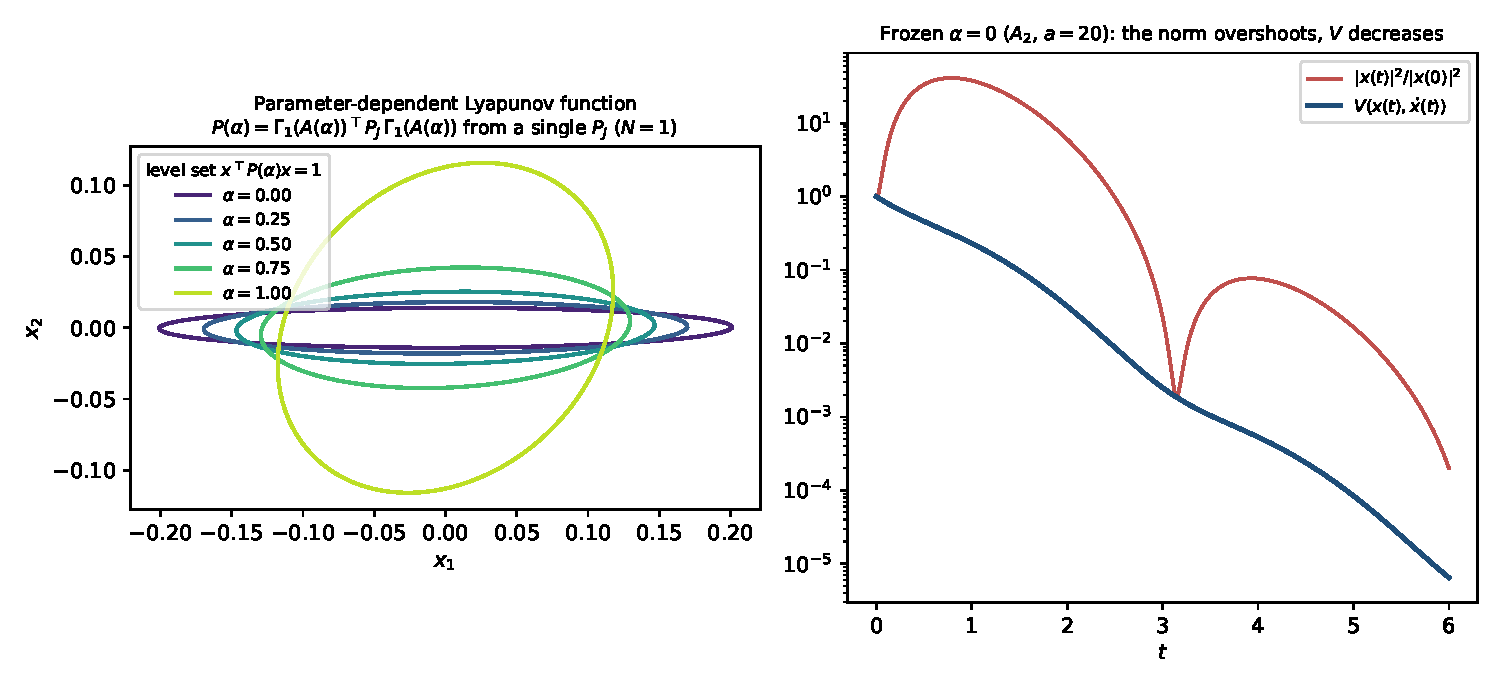
\includegraphics[width=0.8\textwidth]{fig_polytope.pdf}
\small Left: level sets $x\tr P(\alpha)x=1$, $P(\alpha)=\Gamma_1(A(\alpha))\tr\PP\Gamma_1(A(\alpha))$, generated by the single $4\times4$ matrix $\PP$: they rotate and stretch with $\alpha$, from nearly circular at $\alpha=1$ ($A_1$) to very elongated at $\alpha=0$ ($A_2$). Right: along $\dot x=A_2x$ the Euclidean norm overshoots by a factor $40$ (non-normality) while $V(x,\dot x)$ decreases monotonically.
\end{frame}

\begin{frame}{Example 1: the same certificate under a time-varying parameter}
\centering
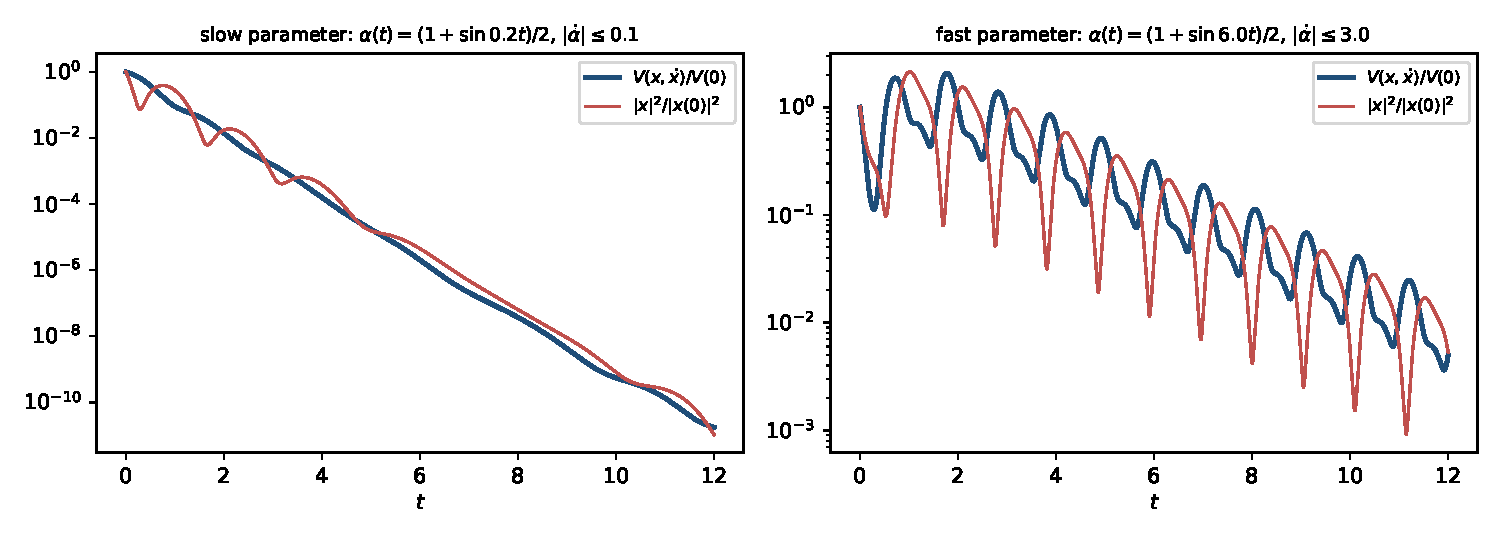
\includegraphics[width=0.9\textwidth]{fig_polytope_tv.pdf}
\small $\dot x=A(\alpha(t))x$, $\alpha(t)=(1+\sin\omega t)/2$, $|\dot\alpha|\le\omega/2$. Left, $\omega=0.2$: $V(x,\dot x)$ (with $\dot x=A(\alpha(t))x$) is monotone, as Corollary 17 predicts for slow variations. Right, $\omega=6$: $V$ is no longer monotone and the decay is visibly slower; the certificate was obtained for constant $\alpha$ and says nothing about fast variations.
\end{frame}

\begin{frame}{Example 2: a polytope that requires level $2$}
\begin{block}{Construction}
Three similar copies $A_i=S_iJS_i^{-1}$ of a non-normal block $J=\begin{pmatrix}-1&b&0\\0&-1&b\\0&0&-1\end{pmatrix}$ with random well-conditioned $S_i$, the strength $b$ increased until the polytope $\co\{A_1,A_2,A_3\}$ reaches the boundary of robust stability, then a time rescaling (entries rounded to two decimals):
\end{block}
\[
A_1=\begin{pmatrix}-0.38&3.58&3.22\\2.32&1.62&1.65\\-3.21&-5.12&-4.72\end{pmatrix},\quad
A_2=\begin{pmatrix}1.63&1.03&1.12\\-10&-0.57&2.74\\4.46&-1.63&-4.54\end{pmatrix},\quad
A_3=\begin{pmatrix}-0.24&4.86&-1.98\\-1.24&-2.42&0.94\\-1.78&1.31&-0.83\end{pmatrix}.
\]
\begin{itemize}
\item Vertices: eigenvalues with real parts in $[-1.5,-0.98]$. Polytope: $\max_{\alpha\in\Delta_3}\max\operatorname{Re}\operatorname{eig}A(\alpha)=-0.024$ (grid of $20\,301$ points): robustly Hurwitz, but with a small margin in the interior.
\item \textbf{Criterion}: the best achievable decrease margin $\gamma^*=\max\{\gamma:\ \text{decrease}\preceq-\gamma I\}$ under the normalization $V\ge|x|^2$ on admissible jets and $\|\PP\|\le10^3$. A certificate exists iff $\gamma^*>0$.
\end{itemize}
\end{frame}

\begin{frame}{Example 2: results}
\begin{center}
\begin{tabular}{lcc}\toprule
 & vertex LMIs with slack variables & exact conditions on a grid of $66$ values of $\alpha$\\\midrule
level $N=0$ & $\gamma^*=-0.97$ & $\gamma^*=-8.19$\\
level $N=1$ & $\gamma^*=-0.38$ & $\gamma^*=-1.30$ (two solvers; unchanged with $\|\PP\|\le10^6$)\\
level $N=2$ & $\gamma^*=+3.61$ & $\gamma^*>0$\\\bottomrule
\end{tabular}
\end{center}
\begin{itemize}
\item The gridded conditions are \emph{necessary} for any quadratic form in the $N$-jet (they are the exact conditions at finitely many $\alpha$): $\gamma^*<0$ at level $1$ proves that \alert{no quadratic form in $(x,\dot x)$ is a Lyapunov function for this family}, whatever the multipliers.
\item At level $2$, the vertex LMIs with constant slack variables are feasible with a comfortable margin: a function $V(x,\dot x,\ddot x)$, i.e.\ $x\tr P(\alpha)x$ with $P(\alpha)$ of degree $4$ in $\alpha$ generated by one $9\times9$ matrix $\PP$.
\item This is the situation the hierarchy is designed for: the order of the jet is the parameter to increase, and Theorem 12 guarantees that some order works.
\item For comparison (same gridded conditions): parameter-dependent functions affine in $\alpha$ give $\gamma^*=-1.81$ (no affine certificate), homogeneous polynomials of degree $2$ in $\alpha$ give $\gamma^*=+5.33$. Consistent with level $1\subset$ degree $2$: the example shows the need for level $2$, not an advantage over polynomial classes.
\end{itemize}
\end{frame}

\begin{frame}{Example 3: a saturated feedback loop}
\begin{block}{The system}
\[
\dot x=Ax+B\sat(Kx),\qquad A=\begin{pmatrix}0.3&1\\-1&0.3\end{pmatrix},\ B=\begin{pmatrix}0\\1\end{pmatrix},\ u_0=1,\ K\approx(-12.86,\,-11.52).
\]
\end{block}
\begin{itemize}
\item Open loop: unstable focus (eigenvalues $0.3\pm i$). With a bounded input the region of attraction of the origin is bounded.
\item $K$ is the LQR gain for $Q=I$, $R=0.01$: a high gain, so the linear region $\mathcal R_0=\{|Kx|\le1\}$ is a thin strip and most of the region of attraction lies where the input saturates. This is where a function of $(x,\psi)$, $\psi=\dz(Kx)$, can differ from a quadratic function of $x$.
\item \textbf{Reference region of attraction}: simulation from a $141\times141$ grid of initial conditions in $[-3,3]^2$, integration over $30$ time units, convergence declared if $|x(30)|<10^{-2}$ and the solution stays bounded.
\end{itemize}
\end{frame}

\begin{frame}{Example 3: what is computed and how}
\begin{enumerate}
\item \textbf{Two certificates from Proposition 26}, same LMIs, same region-wise structure:
\begin{itemize}
\item quadratic: $\PP=\diag(P,0)$, $\mu=0$, $\lambda_b=\lambda_c=0$ --- the generalized sector condition of Gomes da Silva--Tarbouriech;
\item order-one jet: full $\PP\in\R^{3\times3}$, all multipliers free.
\end{itemize}
\item \textbf{Size criterion}: the radius $\beta$ of the largest ball $\{|x|\le\beta\}$ certified inside $\Omega_V=\{V(x,\dz(Kx))\le1\}$.
\item \textbf{Bilinear scalars} $\mu$ (level-set multiplier) and $\lambda_e$ (generalized-sector multiplier): line search on logarithmic grids, $\lambda_e\in[10^{-2},10^{2}]$, $\mu\in\{0\}\cup[10^{-2},10^{1.5}]$; for each pair, bisection on $\beta$; $\varepsilon=10^{-4}$; CVXPY + Clarabel. The best certificate found is reported.
\item \textbf{Plots}: the two level sets $\{V=1\}$ (contours of $V(x,\dz(Kx))$ on a grid), the simulated region of attraction, twelve trajectories from the boundary of the jet estimate, and $V$ along one of them.
\end{enumerate}
\end{frame}

\begin{frame}{Example 3: estimates of the region of attraction}
\begin{columns}
\column{0.48\textwidth}
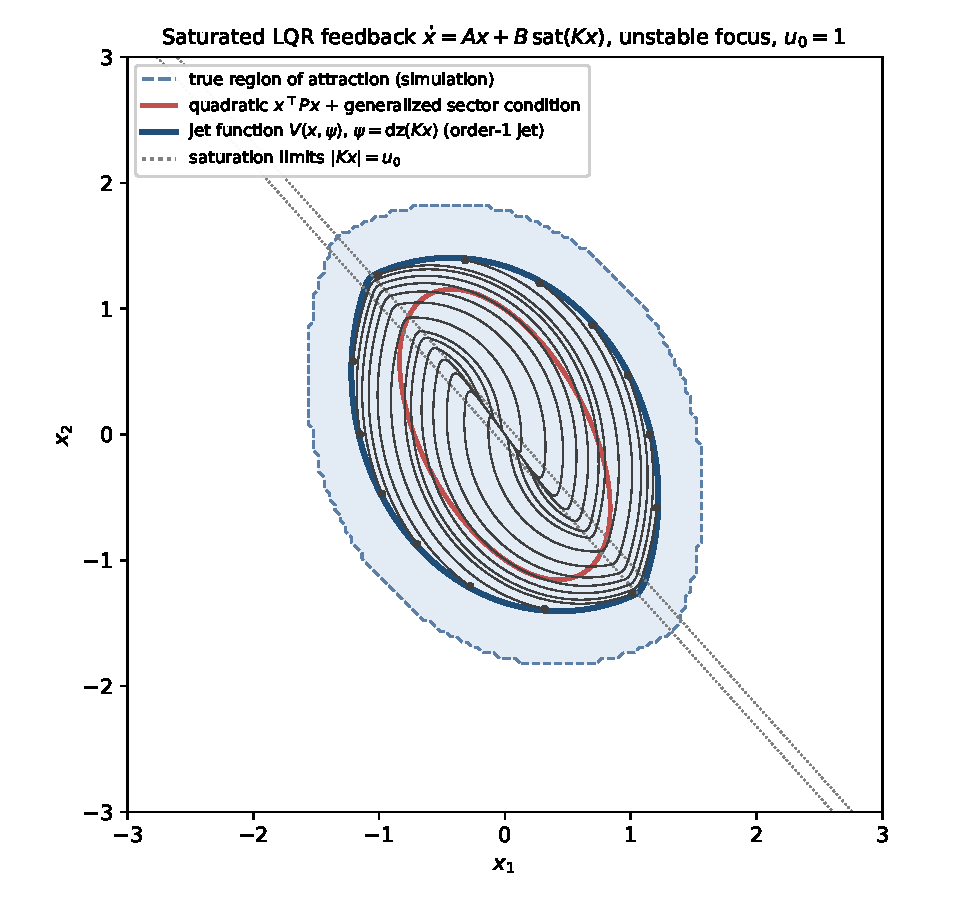
\includegraphics[width=0.92\textwidth]{fig_regional.pdf}
\column{0.52\textwidth}\small
\begin{itemize}
\item Shaded: region of attraction (simulation). Dotted: the saturation lines $|Kx|=u_0$.
\item Red: quadratic estimate with the generalized sector condition, $\beta=0.67$.
\item Blue: order-one jet estimate $\{V(x,\dz(Kx))\le1\}$, $\beta=1.09$. It is not an ellipse: three elliptic arcs glued continuously along the saturation lines (the function is quadratic in $x$ on each region), about three times the area of the red set.
\item Trajectories from the boundary of the blue set stay inside it and converge: the set is forward invariant, as Proposition 26 guarantees.
\end{itemize}
\end{columns}
\end{frame}

\begin{frame}{Example 3: along a trajectory from the boundary of the estimate}
\centering
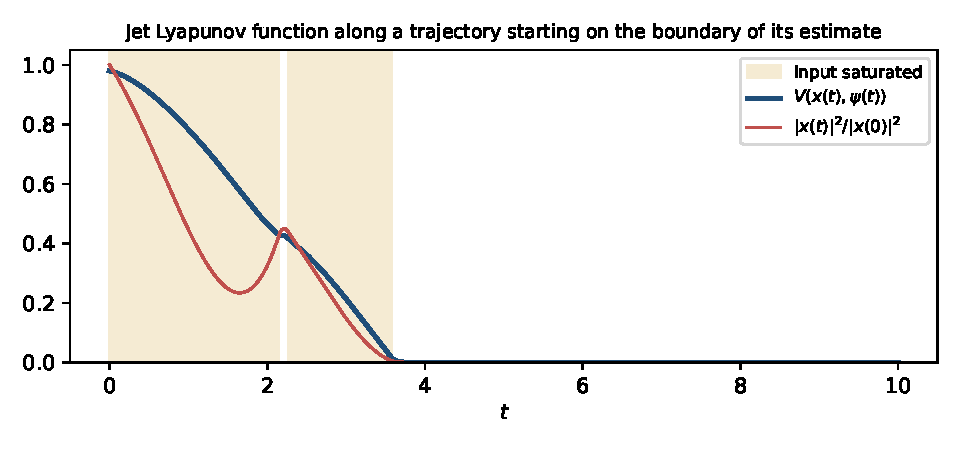
\includegraphics[width=0.9\textwidth]{fig_regional_traj.pdf}
\small $V(x(t),\psi(t))$ (blue) decreases monotonically, with a kink at each crossing of a saturation line (the function is continuous but not differentiable there: the trajectory switches region); the squared norm (red) increases on part of the trajectory. Shaded: intervals where the input is saturated.
\end{frame}

\section{Conclusions and open problems}

\begin{frame}{Summary}
\begin{itemize}
\item \textbf{Framework}: Lyapunov functions on jets; conditions on admissible jets only; Finsler + S-procedure.
\item \textbf{Universal form} $V_{T,N}=\int_0^T|\tau_N|^2$ with the identity $\dot V=|\tau_N(T)|^2-|x|^2+\text{truncation}$.
\item \textbf{Converse theorem}: any compact Hurwitz family admits $V_{T,N}$ as common Lyapunov function; $T$ from the overshoot time, $N$ from $a/\lambda$ and $\ln c$.
\item \textbf{Hierarchy}: nested, asymptotically exact; positivity on admissible jets contains affine PDLFs; size of $\PP$ independent of the number of parameters.
\item \textbf{Slowly varying}: explicit tolerance, non-vanishing as $N\to\infty$; jointly affine constraints in parameter derivatives.
\item \textbf{Analytic families}: order governed by overshoot vs.\ analyticity radius.
\item \textbf{Lur'e}: LMI conditions; conserved quantity of the LPV form.
\item \textbf{Saturation}: order-one ceiling; region-wise LMIs; non-ellipsoidal estimates.
\end{itemize}
\end{frame}

\begin{frame}{Open problems}
\begin{enumerate}
\item \textbf{Constant multipliers.} Is the vertex relaxation with constant $G_0,G$ asymptotically exact as $N\to\infty$? (In the proof of Theorem 7 the constraints are used only to identify $\tau_N(T)$ with $E_N(TA)x$.)
\item \textbf{Rate-bounded converse.} Robust stability for all $|\dot w|\le\delta_0$ $\Rightarrow$ a quadratic form in some jet for all rates below $\delta_0$? Route: converse for rate-bounded systems + jet identifiability (Proposition 14).
\item \textbf{Lur'e systems.} Converse theorem accounting for the conserved quantity; link with Zames--Falb multipliers.
\item \textbf{Beyond the radius of analyticity.} Does $\bigcup_N\mathcal Q_N(f)$ always contain a Lyapunov function on a compact invariant set?
\item \textbf{Non-smooth solutions.} What replaces the jet for differential inclusions? $C^N$ selections and density, or set-valued jets and $W(x)=\sup_{j\in\Jet^N_F(x)}V(j)$.
\end{enumerate}
\end{frame}

\begin{frame}
\centering
\Large Thank you.
\bigskip

\normalsize Questions?
\end{frame}

\end{document}
